\documentclass{article}
\usepackage[]{graphicx}
\usepackage[]{xcolor}
\usepackage{alltt}
\usepackage[left=2.3cm,right=2.8cm, top = 2.2cm, bottom = 3cm]{geometry}
\usepackage{amsmath}
\usepackage{amssymb}
\usepackage{natbib}
\PassOptionsToPackage{hyphens}{url}
\usepackage{url} 
\usepackage[disable]{todonotes}
\usepackage{multicol}
\usepackage{rotating}
\usepackage{booktabs}
\usepackage[colorlinks=false]{hyperref} 
\setlength{\parskip}{\baselineskip}%
\setlength{\parindent}{0pt}%
\urlstyle{same}
\usepackage{lineno}
\linenumbers
\bibliographystyle{apalike}


% to handle authorship footnotes as numbers:
\makeatletter
\let\@fnsymbol\@arabic
\makeatother

\newcommand{\ra}[1]{\renewcommand{\arraystretch}{#1}}
\newcommand{\changed}[1]{#1}

% to write the simulated as iid symbol: 
\newcommand{\distas}[1]{\mathbin{\overset{#1}{\kern\z@\sim}}}%


\begin{document}


\title{To log or not to log}
  \author{Anonymous Alpaca\thanks{All Alpaca friends} $^{,}$\thanks{The Zoo} $^{ , *}$}

\maketitle

\tableofcontents

\begin{abstract}
In the abstract, this article is a very good one. We did a very good job of the research and got all the best results. People told us we were mad and we said no we are effective. Now gather around and listen to our thoughts you will be, shocked, scared, amazed, and astounded.
\end{abstract}

\bigskip

{\footnotesize $^*$ Correspondence to: Anonymous Alpaca (\url{anonymous@alpaca.com}))}



\newpage


% ===========================================================
\section{Introduction}

Probabilistic forecasts play an important role in decision-making in epidemiology and public health \citep{reichCollaborativeMultiyearMultimodel2019, funkShorttermForecastsInform2020, cramerEvaluationIndividualEnsemble2021, bracherShorttermForecastingCOVID192021, europeancovid-19forecasthubEuropeanCovid19Forecast2021, sherrattPredictivePerformanceMultimodel2022}, as well as other areas as diverse as for example economics \citep{timmermannForecastingMethodsFinance2018, elliottForecastingEconomicsFinance2016} or meteorology \citep{gneitingWeatherForecastingEnsemble2005, kukkonenReviewOperationalRegionalscale2012}. Epidemiological modelling in particular has received widespread attention during the COVID-19 pandemic and has been an important tool to inform public policy. Evaluating forecasts is important, as the evaluation provides feedback for forecasters and researchers necessary to improve their models, and it helps decision makers distinguish good from bad predictions and choosing forecasts that inform future decisions.

Proabbilistic forecasts are usually evaluated using so-called proper scoring rules, which return a numerical score as a function of the forecast and the later observed data. Forecasters, in expectaction, optimise their score by providing a predictive distribution that is equal to the data-generating distribution, and will be penalised if they fail to do so. Two proper scoring rules commonly used in epidemiology and other fields are the Continuous Ranked Probability Score (CRPS) \citep{gneitingStrictlyProperScoring2007} and the Weighted Interval Score (WIS) \citep{bracherEvaluatingEpidemicForecasts2021}. Both the WIS and CRPS represent a measure of the absolute distance between the predictive distribution and observation and represent a generalisation of the absolute error to full predictive distributions (see details in the SI). The WIS can be thought of as an approxmiation of the CRPS for forecasts in a quantile format and has very similar properties (the WIS converges towards the CRPS for an increasing set of equally-spaced prediction intervals). Due to its widespread use in epidemiology (and its similarity to the CRPS) we mostly focus on the WIS in this paper, ignoring other proper scoring rules. Formulas for the WIS are given in the SI. 

% Maybe insert WIS formula here? 

Evaluating forecasts based on absolute errors (for simplicity we use the term interchangeably with absolute distance, even though the former technically only applies to point forecasts), as is done by the WIS, may not always be desirable, especially in an epidemiological context. 
% The reason for this is that generally, the way for ecasts are evaluated should correspond to the error structure of the model and the type of errors models will usually make.
Epidemiological processes are usually understood to be exponential in nature and therefore are most commonly described and modeled in multiplicative terms. Under the assumption that these models are correctly capturing the underlying inherent transmission dynamics, it would therefore make sense to focus evaluation on multiplicative, rather than absolute errors. Often, if the model is performing badly in multiplicative terms, this means that there is a flaw with its assumptions that needs to be resolved, regardless of performance in absolute terms. Evaluating epidemiological forecasts based on a measure of absolute error (as is common practice) can make it harder to diagnose and quantify model mis-specification. It also may make it more difficult to deal with the potential non-stationarity of epidemiological processes, or to compare performance across targets that are on very different orders of magnitudes (like for example cases and hospitalisations). 

In this paper we argue that it may therefore be helpful to shift the focus of the evaluation on multiplicative, rather than absolute errors. This is approximately equal to scoring the growth rate of a forecast and can be achieved by transforming the forecasts as well as the observations using the logarithm before applying the WIS or CRPS. We focus on the log transformation, as it represents a very convenient way of achieving our goal of evaluating how well a forecast captures the growth dynamic inherent to epidemiological process. However, we note that the same logic we use can also applied to other transformations which could shift the focus of evaluation in different ways. For example, given an appropriate transformation, it could also be possible to evaluate forecasters based on the shape of the trajectory they predicted. It would even be possible to construct composite scores as a weighted sum of scores based on different transformations, allowing forecast consumers to assign explicit weights to different qualities of the forecasts. 

In section [REF] we discuss the broader idea of transforming forecasts, and in section [REF] give a detailed theoretical of the log transformation and its interpretation. In section [REF] we present an applied example using forecasts submitted to the European COVID-19 Forecast Hub \citep{europeancovid-19forecasthubEuropeanCovid19Forecast2021, sherrattPredictivePerformanceMultimodel2022}. The European COVID-19 Forecast Hub is one of several Forecast hubs (together with a Hub in the US \citep{cramerEvaluationIndividualEnsemble2021} and one in Germany and Poland \citep{bracherShorttermForecastingCOVID192021} that systematically collected, aggregated and evaluated forecasts of several COVID-19 targets created by different teams. Forecasts submitted to the COVID-19 Forecast Hubs are probabilistic in nature [Citation e.g. Held et al.], meaning that forecasters provide a full predictive distribution which quantifies their uncertainty. These predictive distributions are reported in the form of a set of 23 quantiles (11 symmetric prediction intervals as well as a median prediction). 
%Currently, the US Flu Forecasting Hub and COVID-19 Scenario Hubs in the US and in Europe use the same format. 

%%%%%%%%%%%%%%%%%%%%%%%%%%%%%%%%%%%%%%%%%%%%%%%%%%%%%%%%%%%%%%%%%%%%%%%%%%%%
\section{Log transforming forecasts and observations}

Applying the log transformation, among other transformations, is permissible because it is a strictly monotonic transformation. While rankings between different models may indeed change, even for a single forecast, the relevant condition for a scoring rule to be strictly proper is still satisfied: In expectation a forecaster will receive the best score if she reports a predictive distribution that is equal to the data-generating distribution, even after transforming both the forecasts and the observations (representing draws from the data-generating distribution). 

It is important to first apply the transformation and then score the transformed forecasts and observations. Simply taking the log of the WIS or the CRPS computed on the natural scale, i.e. computing $\log S(x, y)$ results in an improper score and is therefore not advised. This is because the logarithm of the WIS / CRPS does not penalise outliers enough and therefore incentivises overconfident predictions. We illustrate this point using simulated data in Figure \ref{fig:log-improper}, where it can easily be seen that overconfident models perform best in terms of the log WIS. 

\begin{figure}[h!]
    \centering
    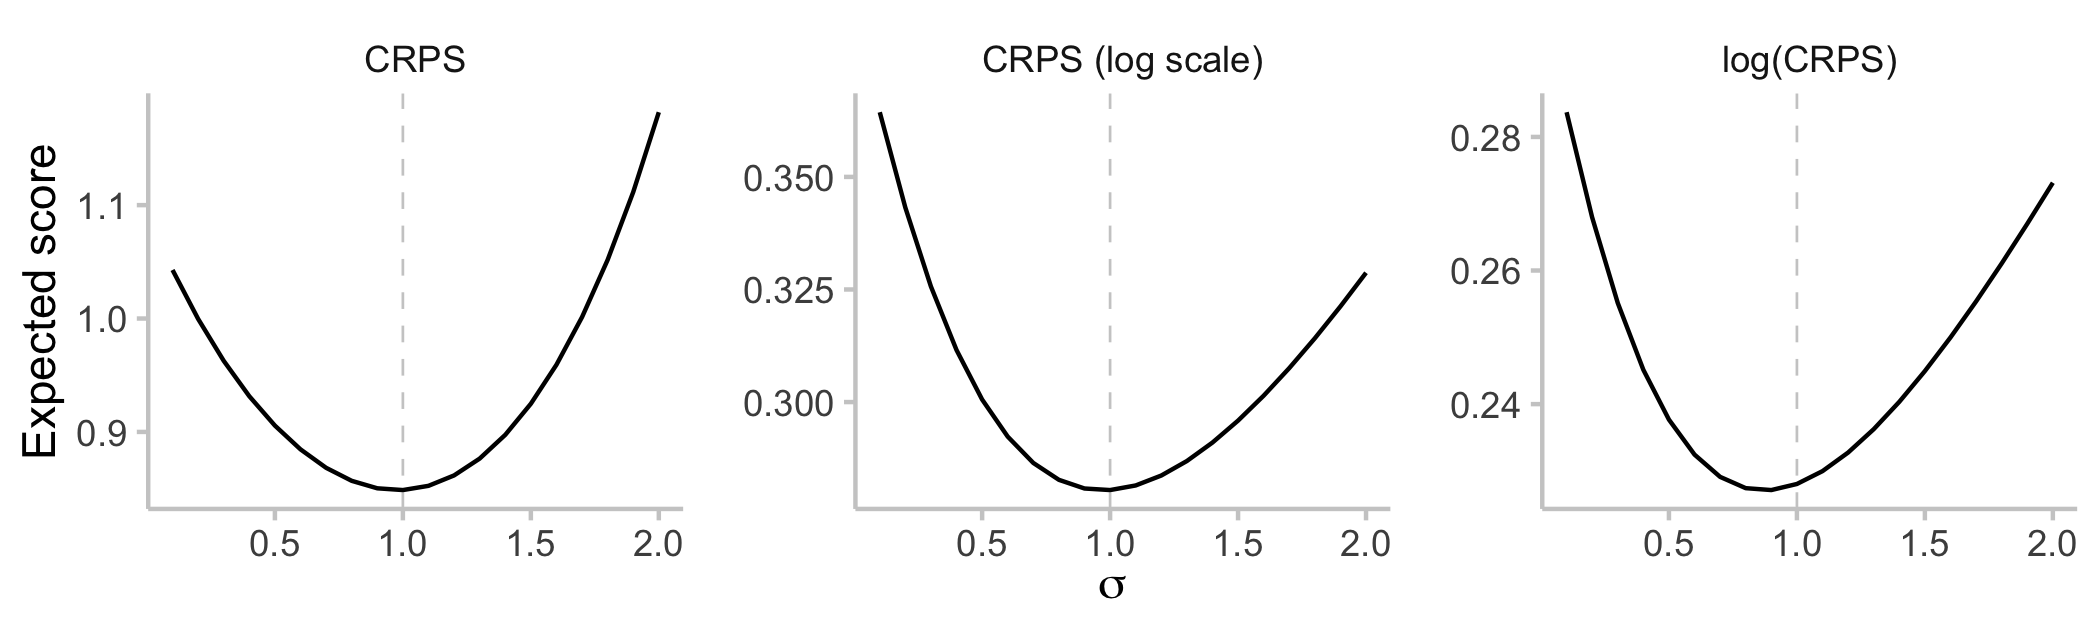
\includegraphics[width=0.9\textwidth]{output/figures/example-log-first.png}
    \caption{Scores for different forecasts evaluated the WIS and the log WIS. We simulated 1000 observations $Y_i = {\rm e}^{x_i}$, with $x_i \text{iid} \sim \mathcal{N}(0, 1)$. We then simulated 20 forecasters who would issue a predictive distribution $F = {\rm e}^{x_i}$, with $x \sim \mathcal{N}(0, \sigma)$, with values of $\sigma$ ranging from 0.1 to 2.}
    \label{fig:log-improper}
\end{figure}


Unfortunately, the log transformation cannot readily be applied when dealing with negative or zero values. In an epidemiological setting that involves count data, negative values should likely be omitted entirely. Values of zero should potentially also be removed from the analsys, as it does not make sense to interpret relative errors on zero counts. Alternatively, if one is not willing to omit them, a small quantity (such as 1) could be added to all observations before taking the logarithm. Note that predictive distribtions have to be truncated in a similar way. When dealing with count data we could extend this argument to all small values (rather than just zeros), as it is hard to reliably evaluate relative errors when dealing with small discrete values. One could therefore decide to remove forecasts for small quantities below a certain threshold from the analysis. 

\subsection{Scoring multplicative errors}

To illustrate the effects of applying the logarithm intuitively, let us consider a point forecast $\hat{y}_{t+1}$ for a quantity of interest $y_{t+1}$, such that 
\begin{equation}
y_{t+1} = \hat{y}_{t+1} + \varepsilon_{t+1}.
\end{equation}

The analogon of the WIS / CRPS for point forecasts is the absolute error, and so the score will be determined by the size of the forecast error $\varepsilon_{t+1}$. When taking the logarithm of the forecast and the observation first, then the score is determined based on the size of $\varepsilon^*_{t+1}$: 
\begin{equation}
\log y_{t+1} = \log \hat{y}_{t+1} + \varepsilon^*_{t+1}.
\end{equation}
%
It is easy to see that this corresponds to evaluating a multiplicative error on the original $y_{t+1}$:
%
\begin{align}
\log y_{t+1} &= \log \hat{y}_{t+1} + \varepsilon^*_{t+1} \Leftrightarrow \\    
y_{t+1} &= \hat{y}_{t+1} \cdot \exp{\varepsilon^*_{t+1}}.    
\end{align}
% %>% 

On the natural scale, WIS and CRPS increase linearly with increasing absolute errors (see Figure \ref{fig:change-in-scores}A, regardless of whether the error is large in relative terms. Predicting 101,000 cases instead of the true 100,000 will be treated equally to predicting 2,000 hospitalisations, rather than the 1,000 observed. On the log scale, WIS and CRPS penalise relative errors and increase linearly with an increase in relative errors (see Figure \ref{fig:change-in-scores}D). Forecasting 101,000 rather than 100,000 cases will be treated equally to forecasting 2,020, rather than 2,000 hospitalisations. While the absolute error on the log scale is exactly symmetric (e.g., predicting 2 instead of 1 would give the same error as predicting 0.5), this is not entirely true for the WIS. Due to the fact that upper and lower bounds of individual prediction intervals are affected differently, there may be slight deviations (compare e.g. in Figure \ref{fig:change-in-scores}D the scores for a relative error of $\frac{1}{5}$ and 5). 

\begin{figure}[h!]
    \centering
    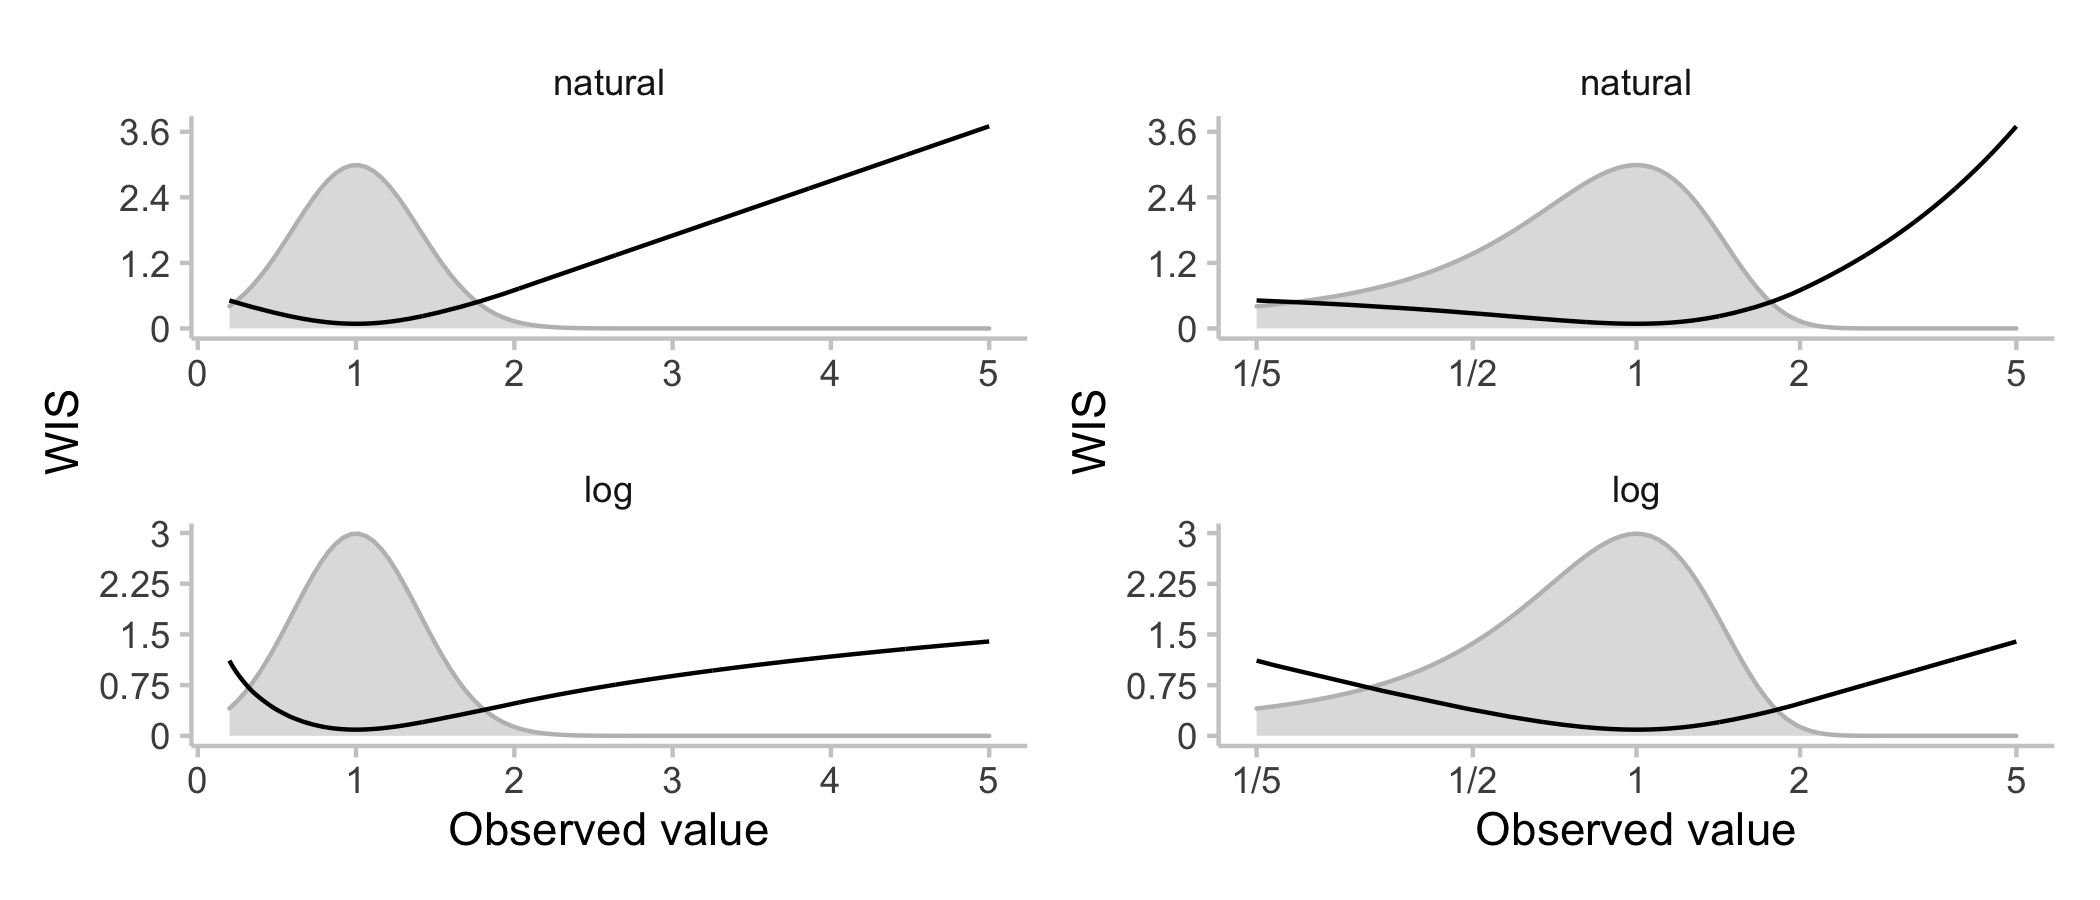
\includegraphics[width=0.9\textwidth]{output/figures/SIM-effect-log-score.png}
    \caption{Weighted interval score for a forecast distribution that is N(1, 0.2) and different observed values. Top: difference in absolute terms. Bottom: difference in relative terms. Interesting panels are top left and bottom right.} 
    \label{fig:change-in-scores}
\end{figure}

\subsection{Approximately scoring the growth rate}
Computing a score based on the logarithm of the forecast and the observation is also approximately equivalent to scoring a forecast of a multiplicative growth rate of the forecast target. The growth rate is defined as
%
\begin{equation}
    g_{t, t+1} = \frac{y_{t+1} - y_t}{y_t},
\end{equation}
%
where $y_{t+1}$ is the forecast target (e.g. reported cases of COVID-19) in the future, $y_t$ is the last known observation and $g_{t, t+1}$ is the growth rate between now ($t$) and $t+1$. 
Using the growth rate, we can express the value of the forecast target in the future as such: 
%
\begin{equation}
y_{t+1} = (1 + g_{t, t+1}) \cdot y_t.
\end{equation}
%

Now consider a forecast on $\log y_{t+1}$. Using the fact that for small values of $x$, $\log (1+ x) \approx x$, we can see that scoring forecasts on the log scale is approximately equal to scoring an additive error on the growth rate (on the natural scale), as long as the growth rate is small.
%
\begin{align}
\log y_{t+1}        &= \log \hat{y}_{t+1} + \varepsilon^*_{t+1} \\
                    &= \log ((1 + \hat{g}_{t+1}) \cdot y_{t}) + \varepsilon^*_{t+1} \\
                    &= \log (1 + \hat{g}_{t, t+1}) + \log y_t + \varepsilon_{t+1} \Leftrightarrow \\
\varepsilon'_{t+1}  &= \log y_{t+1} -  \log y_t - \log (1 + \hat{g}_{t, t+1}) \Leftrightarrow \\    
                    &= \log (\frac{y_{t+1}}{y_t}) - \log (1 + \hat{g}_{t, t+1}) \Leftrightarrow \\    
                    &= \log (1 + g_{t, t+1}) - \log (1 + \hat{g}_{t, t+1}) \Leftrightarrow \\   
                    &\approx g_{t, t+1} - \hat{g}_{t, t+1} \quad \text{for small differences between } \hat{g}_{t, t+1} \text{ and } g_{t, t+1}. 
\end{align}

This approximation breaks down when the difference between the predicted and the actual growth rate becomes too large (albeit forecasts are still evaluated in terms of relative errors). If this is of great concern one may want to use a different transformation like dividing forecasts and observations by the last known values instead in order to score the growth rate explicitly (although this lacks the elegance of having one single transformation per time point). 

Conveniently, the decomposition of the WIS into dispersion, overprediction and underprediction is preserved. The interpretation of the components has now changed in that they now (approximately) represent uncertainty, over-prediction, and under-prediction with the growth rate and so are independent of current incidence. 

\subsection{Effects on model rankings}
Rankings between different forecasts may be affected by applying the log transformation even when looking at a single forecast. As an example, consider two forecasters, A and B. Both issue a single 50\%-prediction interval for a target which later resolves as 1. Forecaster A issues the interval [0.5, 2], while forecaster B issues [0.9. 2.5]. On the natural scale, the score would equal the dispersion of the forecast, i.e. the length of this interval (since the observed value falls within the prediction interval). Forecaster A would receive a score of $2 - 0.5$ = 1.5, beating forecaster B who would receive a score of $2.5 - 0.9 = 1.6$. When we transform the forecast, forecaster A receives a score of $\log (\frac{2}{0.5}) = 1.39$, while forecaster B obtains a score of $\log (\frac{2.6}{0.9} = 1.06$ and now wins over forecaster A. The main difference between forecaster A and B is that forecaster A has issued a prediction interval ([0.5, 2]) that was more symmetric around the true value than the interval issued by forecaster B ([0.9. 2.6], which was more skewed). This means that in relative terms, Forecaster B was noticeably closer to the true value with the lower bound of her prediction interval, while only being slightly further away with the upper interval. This is likely to lead to a more lenient treatment of (one-sided) outlier forecasts. 

Overall model rankings usually differ even more when performance is averaged across multiple forecasts. This effect is not mainly driven by the kinds of changes in model rankings for single forecasts we just discussed. Rather, aggregate scores across multiple forecasts are affected by the fact some scores will in general be much larger than others. On the natural scale, aggregate scores will usually be dominated by predictions of quantities with high absolute values. Even an ideal forecaster will make much larger errors when predicting a quantity such as reported case numbers, than when predicting hospitalisations. Evaluating forecasts based on relative errors may help with comparing performance across different targets. However, log transforming forecasts and observations may also result in the opposite extreme, since small absolute errors (e.g. predicting 9, rather than 3 deaths) may be large in relative terms if the quantity to forecast is very small. This is especially true when forecasts are restricted to discrete values. 
Whether or not forecast targets with smaller quantities receive higher scores than those for targets with larger quantities, depends on the exact relationship between the mean and the variance of the quantity of interest. 

MAYBE MOVE TO SI
For simulated negative binomial count data, log predictions for small quantities receive on average higher scores than forecasts for large quantities if the mean and the variance grow at the same rate $\sigma^2 = \mu$, about equal scores when the variance grows at a rate of $\sigma^2 = \mu + \mu^2$ (Figure \ref{fig:SIM-wis-state-size-mean}), and smaller scores when the variance grows faster than that. 
% To illustrate this with count data we sampled forecasts from different negative binomial distributions. The negative binomial distribution has mean $\mu$ and variance $\sigma^2 = \mu + \mu ^2 / \theta$ and for $\lim_{\theta \to \infty}$ converges to the Poisson distribution. For large values of $\theta$, resulting in a variance approximately equal to the mean, forecasts for lower quantities on average received higher scores on the log scale (see Figure \ref{fig:SIM-wis-state-size-mean}. For $\theta = 1$ (and correspondingly, $\sigma^2 = \mu + \mu^2$, we found that scores on the log scale remained approximately constant regardless of the size of the quantity to forecast. For $\theta = 0.1$ (and $\sigma^2 = \mu + 10 \cdot \mu^2$), scores on the log scale increased with the quantity to forecast. When scored on the natural scale, a higher quantity to forecast always lead to higher scores regardless of the chosen distribution (as long as the variance grows together with the mean). 

I KNOW YOU ALL ARE GOING TO HATE THIS, BUT IT IS SOOOO CLEVER! :-(
If one finds that average scores are dominated by forecasts for small quantities one could omit these forecasts entirely, arguing that relative errors are difficult to meaningfully interpret for small quantities. One might also take a more experimental route, namely adding a number $n$ (e.g. $n = 100$) to all observations and forecasts before taking the logarithm. This also constitutes a strictly monotonic transformation which preserves propriety and would reduce all scores (through reducing relative errors). Scores for forecasts on small quantities would be particularly affected, resulting in a more equal distribution of scores for forecasts of differing orders of magntitudes. Researchers could choose to add either a small or large number, depending on how much they want to equalise relative errors when aggregating scores. 

\begin{figure}[h!]
    \centering
    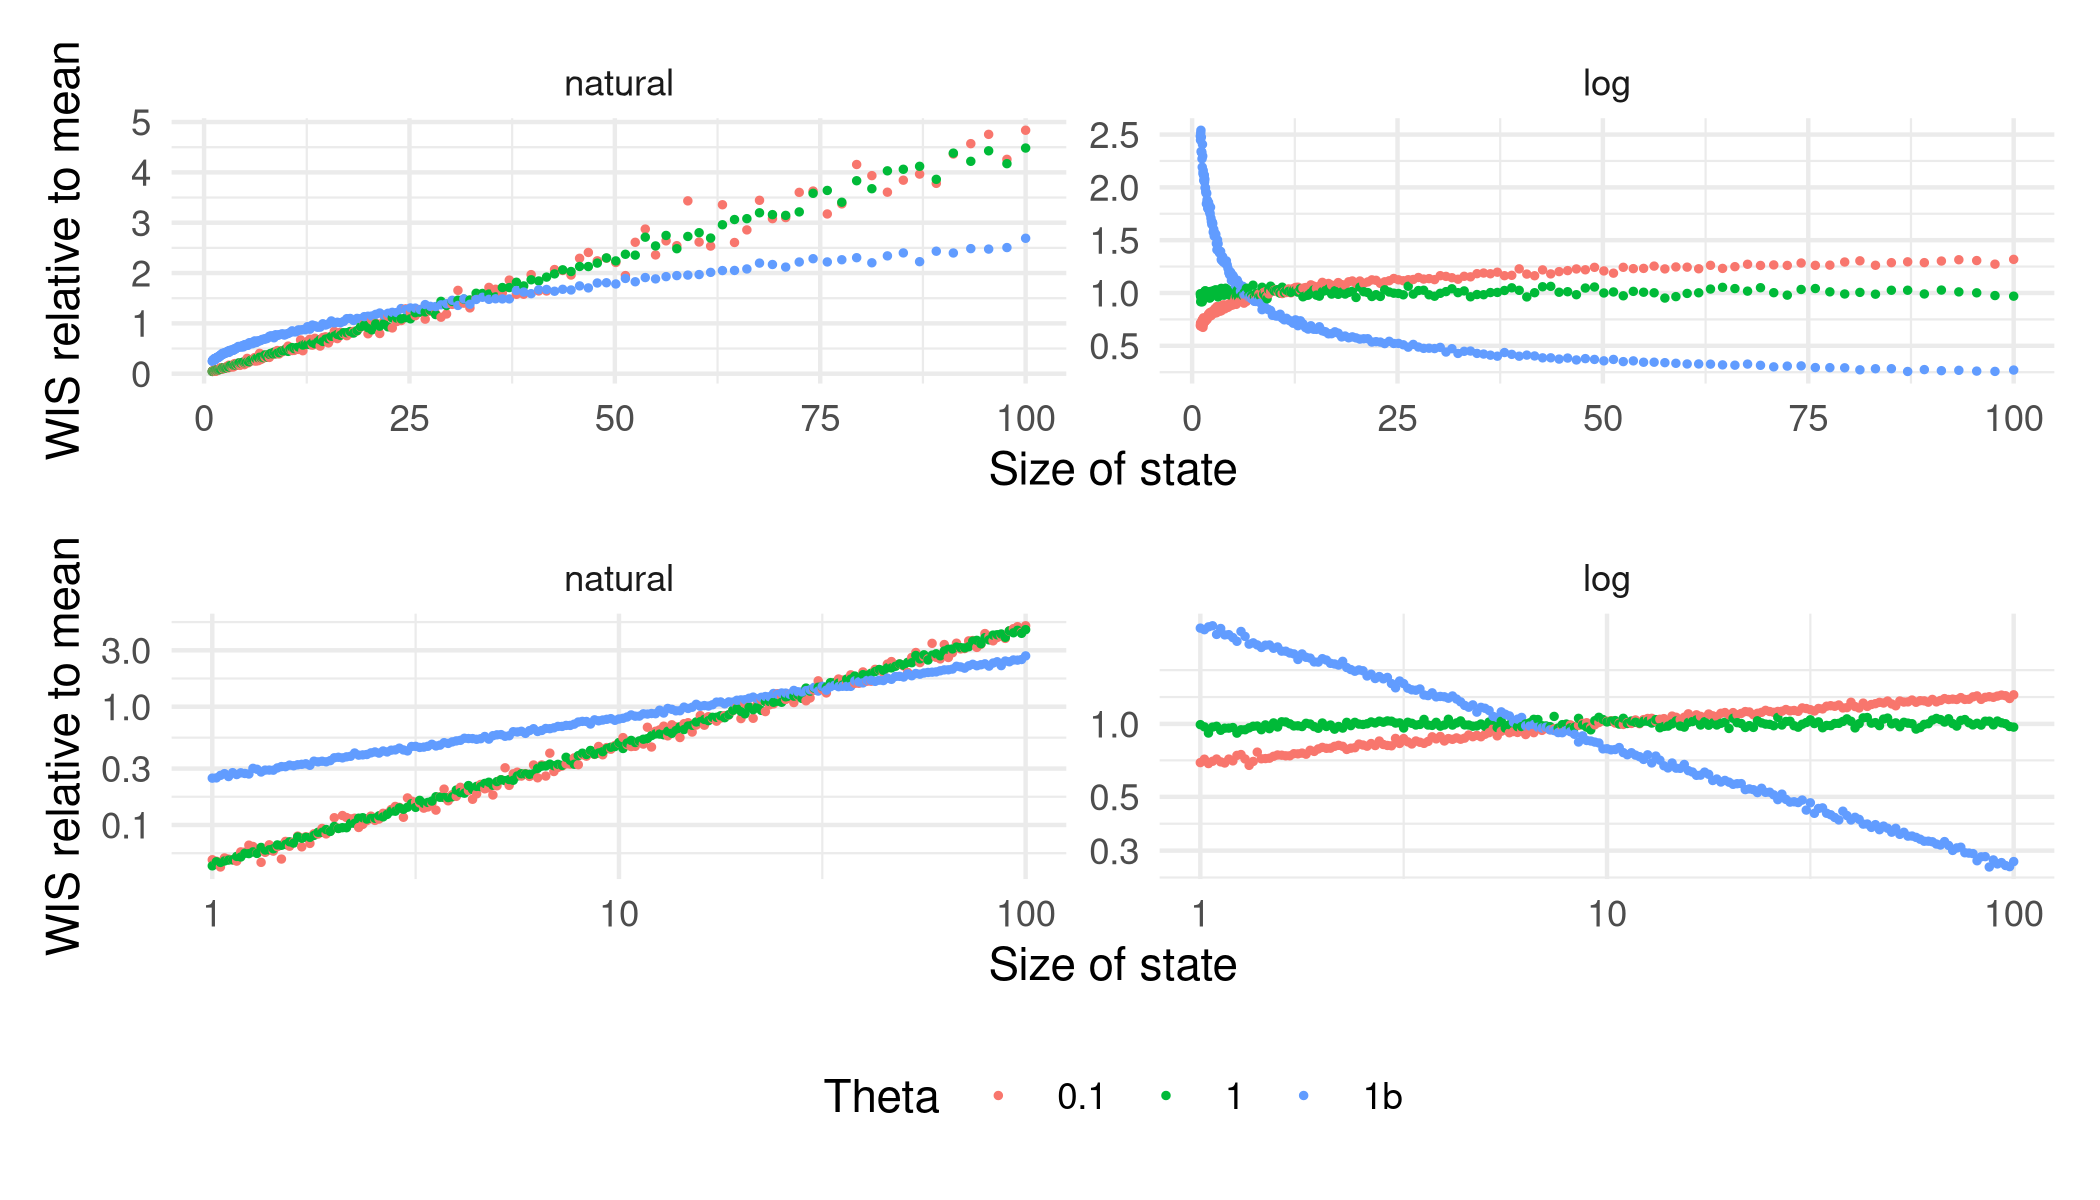
\includegraphics[width=0.9\textwidth]{output/figures/SIM-mean-sd-state-size.png}
    \caption{Simulation of the effect of population size with ideal forecasts of a negative-binomially-distributed variable. For each simulated state, we drew 1,000 observations from a negative binomial distribution with $\mu = 100 \cdot \text{state size}$ and with values of $\theta$ equal to 0.1, 1, and 1 billion. The variance of the negative binomial is given as $\sigma^2 = \mu + \mu^2 / \theta$, meaning that for large theta the negative binomial distribution is equal to the poisson distribution. For these simulated values we computed the WIS for an ideal forecast (i.e. the predictive distribution was negative binomial with $\mu$ and $\theta$ equal to the true $\mu$ and $\theta$ for every state). Left: Mean WIS depending on state size, right: Mean WIS depending on state sizes when scored on a log scale. Plots for the standard deviation, rather than the mean of WIS values look are given in Figure \ref{fig:SIM-wis-state-size-sd} in the SI.}. 
    \label{fig:SIM-wis-state-size-mean}
\end{figure}


%Score different things from the European / US Forecast Hub and plot the relationship between mean and variance. Plot log-scale scores for different things and see which of these influence average scores most \\
% What happens to the decomposition of the WIS if we log? 

%\begin{itemize}
%    \item Optional: Discussion of parallels to point forecasts and the point that you're still incentivised to report the median\\
%\end{itemize}

\section{Empirical example: the European Forecast Hub}

As an empirical example for evaluating forecasts on the natural and on the log scale we use forecasts from the European Forecast Hub \citep{europeancovid-19forecasthubEuropeanCovid19Forecast2021, sherrattPredictivePerformanceMultimodel2022}. Every week the European Forecast Hub collates and aggregates forecasts for different COVID-19 related targets from teams around the world. Forecasts are made one to four weeks ahead into the future and follow a quantile-based format with a set of 22 quantiles plus the median ($0.01, 0.025, 0.05, ..., 0.5, ... 0.95, 0.975, 0.99$). The forecasts for the purpose of this illustrations are two-week-ahead forecasts made between XXX and XXX for reported cases and deaths from COVID-19 in XXX countries. We filtered all forecasts submitted to the Hub to only include models which have submitted forecasts for both deaths and cases for 4 horizons in 32 locations on at least 16 forecast dates. Where not otherwise stated, we report results for a two-week-ahead forecast horizon. 


\begin{table}[h!]
    \centering
    
    \begin{tabular}{lllcc}
    \toprule
    target\_type & quantity & measure & natural & log\\
    \midrule
    Cases & Observations & mean & 20308 & 8.39\\
    Cases & Observations & sd & 43405 & 2.11\\
    Cases & Observations & var & 1884002308 & 4.46\\
    \addlinespace
    Deaths & Observations & mean & 259 & 3.79\\
    Deaths & Observations & sd & 532 & 2.11\\
    Deaths & Observations & var & 283492 & 4.46\\
    \addlinespace
    \hline
    \addlinespace
    Cases & WIS & mean & 4544 & 0.28\\
    Cases & WIS & sd & 17585 & 0.49\\
    \addlinespace
    Deaths & WIS & mean & 28 & 0.22\\
    Deaths & WIS & sd & 67 & 0.26\\
    \bottomrule
    \end{tabular}
    
    \caption{Table with summary statistics for observations and scores for forecasts from the ECDC data set.}
    \label{tab:HUB-summary}
\end{table}

Pooled across all time points and locations, the mean number of cases (deaths) observed was 22811 (368) with an overall standard deviation of 47135 (831) (see Table \ref{tab:HUB-summary}). The average number of observed cases and deaths varies considerably by location (see Figure \ref{fig:HUB-mean-locations}A and B). Observations are overdispersed, meaning that for a given location, the variance in observations exceeds the mean of all observed values (see Figure \ref{fig:HUB-variance-mean}). 
%maybe make a line of best fit of the form variance = alpha * mean^2 + beta * mean

\begin{figure}[h!]
    \centering
    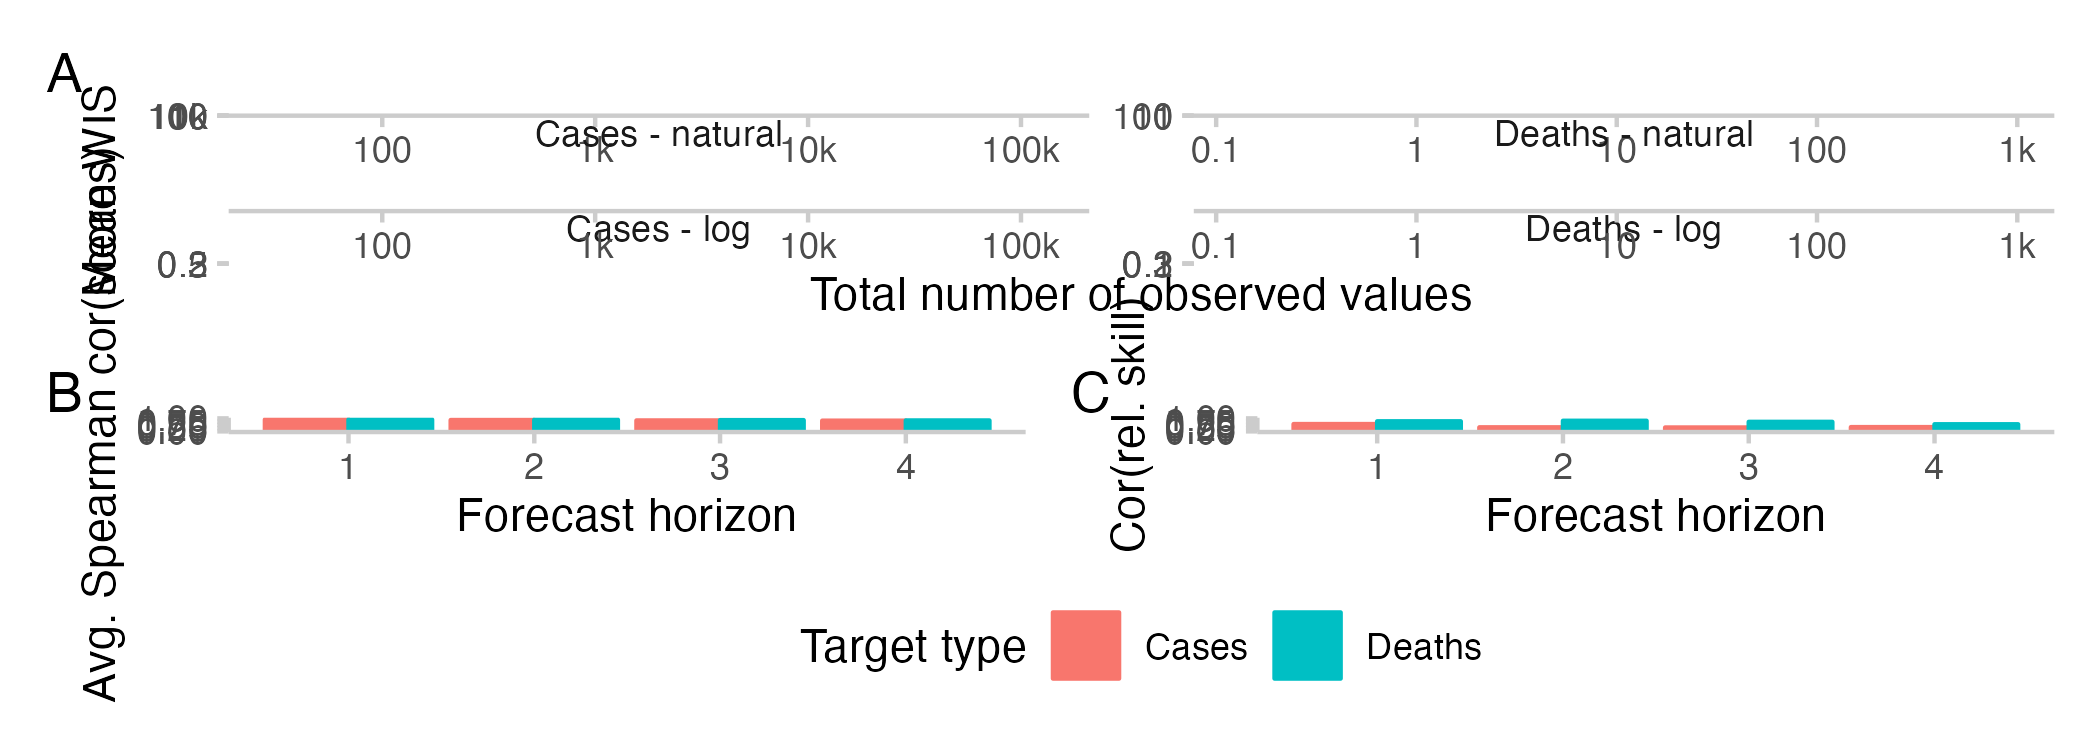
\includegraphics[width=0.9\textwidth]{output/figures/HUB-average-scores.png}
    \caption{Distribution of interval scores for two week ahead forecasts of COVID-19 cases and deaths evaluated on the natural scale (left) and on the log scale (right). }
    \label{fig:HUB-average-scores}
\end{figure}

Pooled across all time points and locations, the mean WIS on the natural scale for cases (deaths) was 8855 (59.3) with an overall standard deviation of 51274 (156) (see Table \ref{tab:HUB-summary}). On the log scale, scores were much closer to each other (see Figure \ref{fig:HUB-average-scores}), with a mean WIS for cases (deaths) of 0.507 (0.362) with an overall standard deviation of 0.745 (0.407). 

Variation of scores across targets (see Figure \ref{fig:HUBXXX} and locations (see Figure \ref{fig:HUB-mean-locations}A, B) is much larger on the natural than on the log scale, where scores are more evenly distributed. On the natural scale, average scores per location correlate strongly (XX) with the average number of observed cases or deaths (See Figure XX). On the log scale, this correlation is much weaker and slightly negative. Forecasts across different locations receive more similar scores, with a tendency for scores to be slightly higher in locations with few observed cases and deaths (see Figures XX and \ref{fig:HUB-mean-locations}. 
%This is in line with the observation that the association between variance is smaller than mu^2 + mu, meaning that we would expect this. 
For individual forecasts, rankings between models are mostly preserved (correlation: X for cases, Y for deaths), with differences increasing across forecast horizons (see Figure \ref{fig:HUB-cors}). 

\begin{figure}[h!]
    \centering
    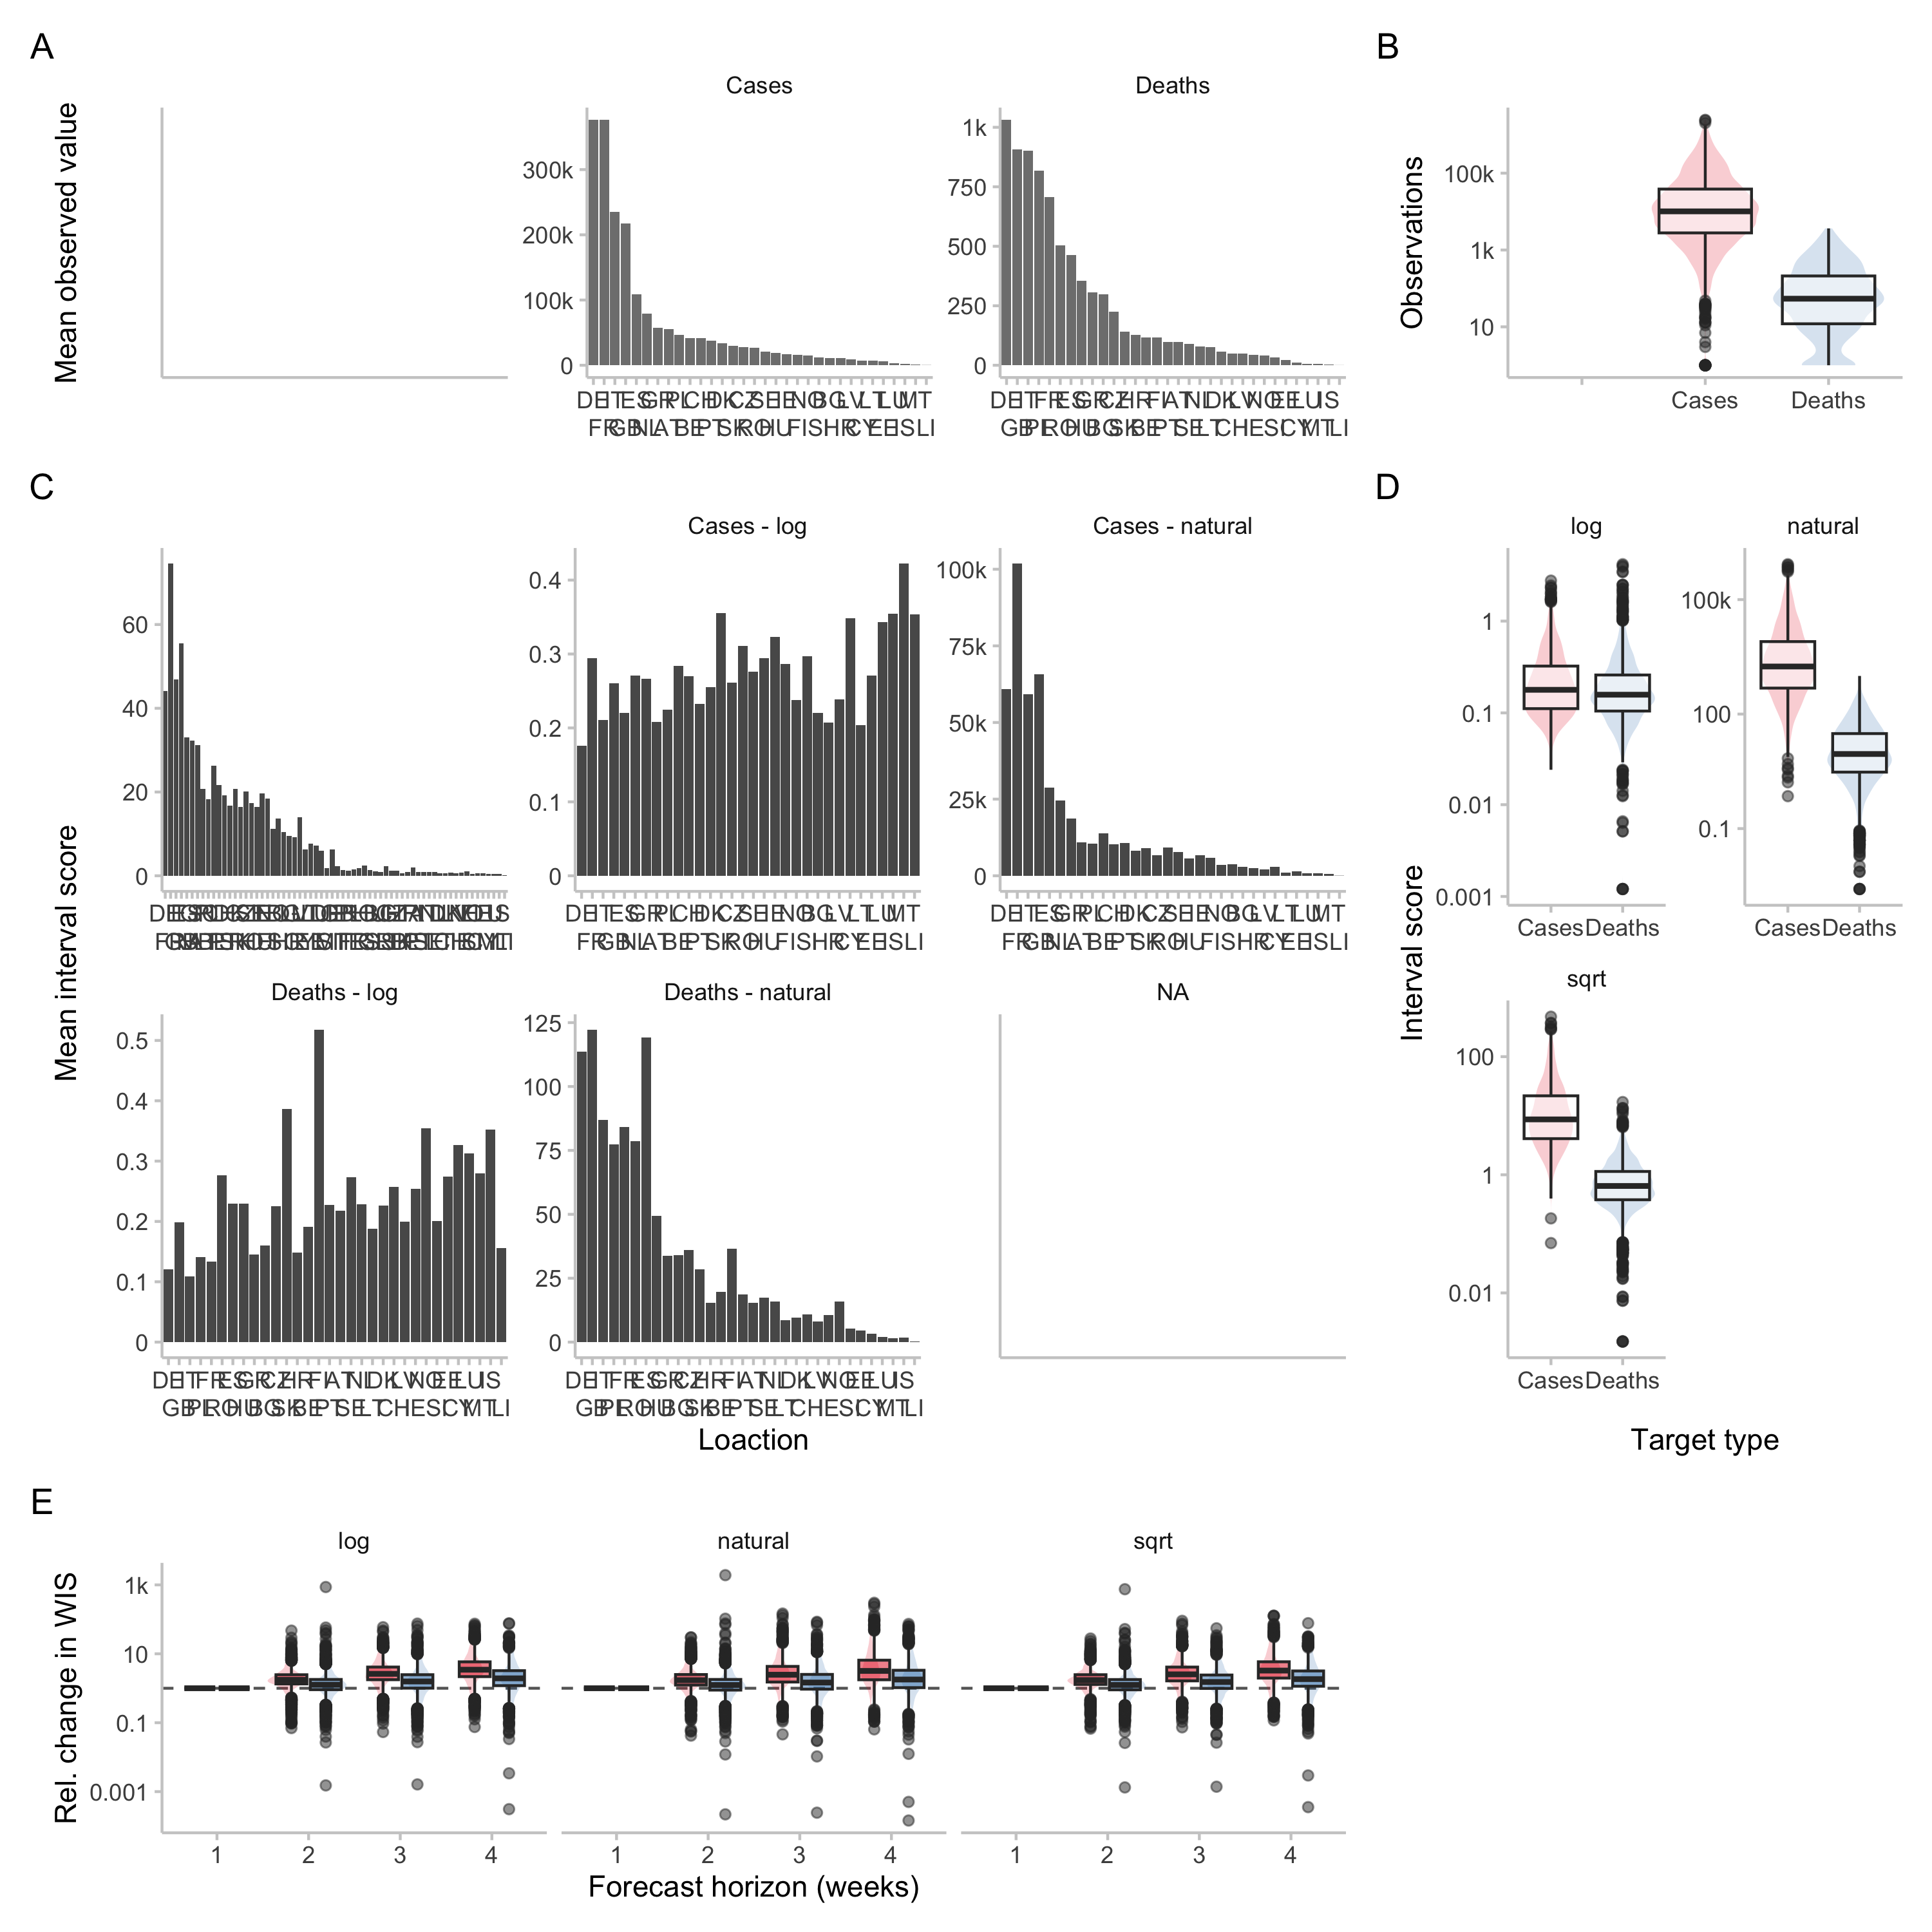
\includegraphics[width=0.9\textwidth]{output/figures/HUB-mean-obs-location.png}
    \caption{Scores and average observed values across 1ocations. A, B: Mean of observed cases and deaths across all time points for different locations. C, D: XXX WIS for forecasts made by the Hub ensemble. D, E: Average WIS for log-transformed forecasts. }
    \label{fig:HUB-mean-locations}
\end{figure}

\begin{figure}[h!]
    \centering
    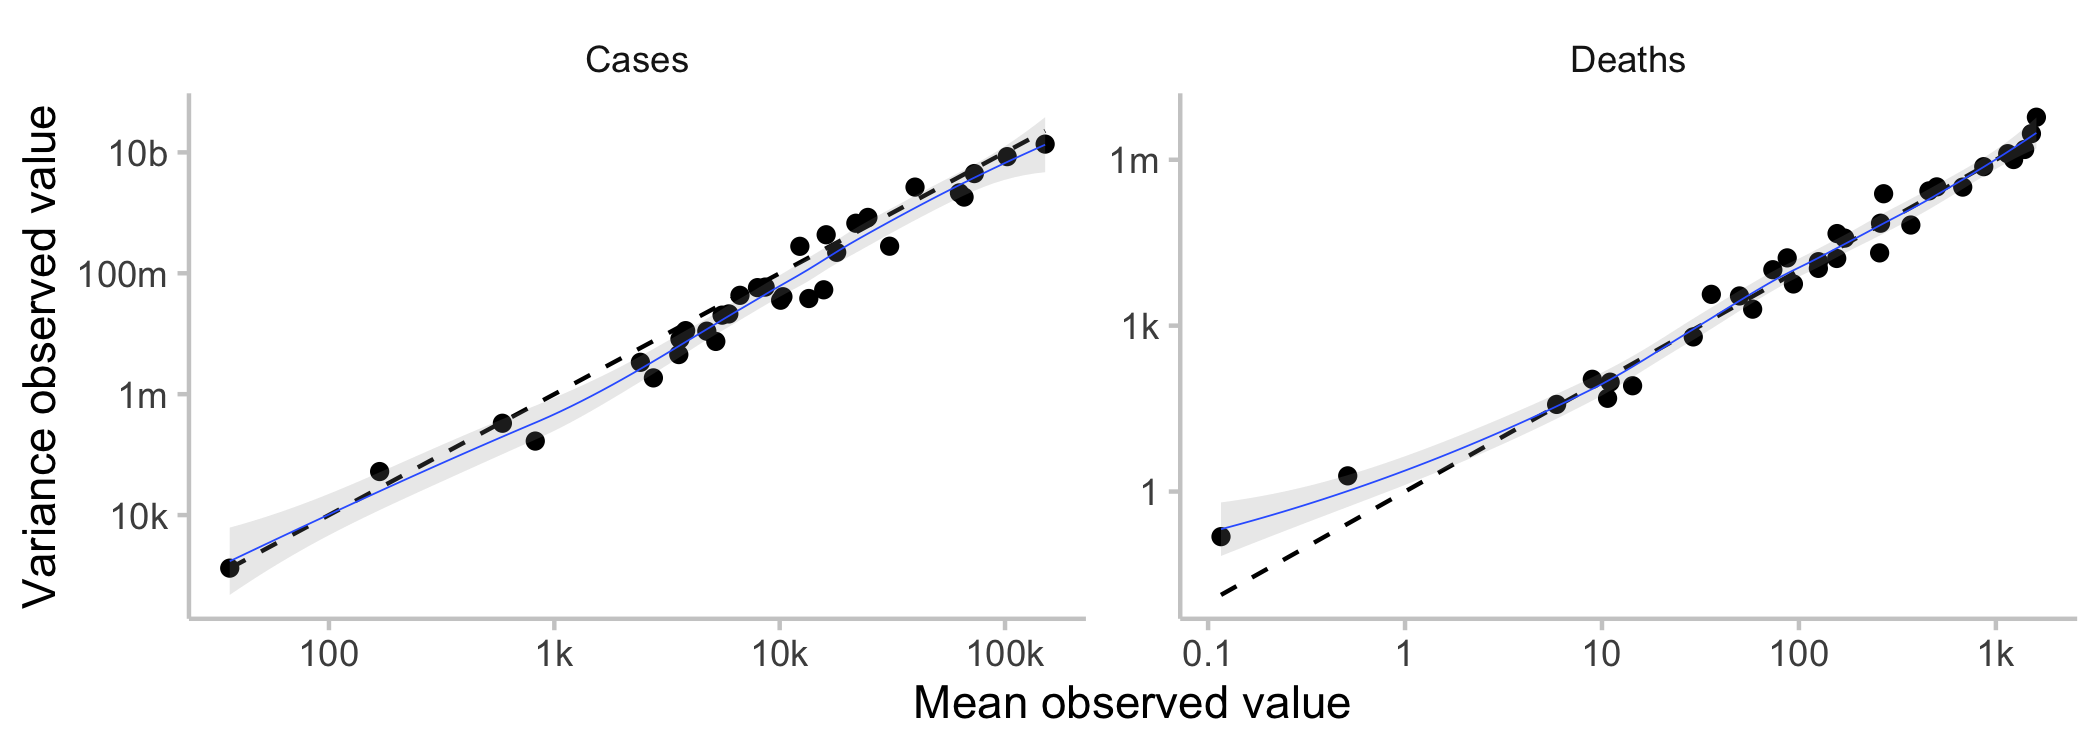
\includegraphics[width=0.9\textwidth]{output/figures/HUB-mean-var-obs.png}
    \caption{Observed mean against observed variance of observations in different locations across time. The dashed line marks what would be expecetd from a negative binomially distributed variable with variance of the observed value equal to the mean + the square of mean observed value. }
    \label{fig:HUB-variance-mean}
\end{figure}

\begin{figure}[h!]
    \centering
    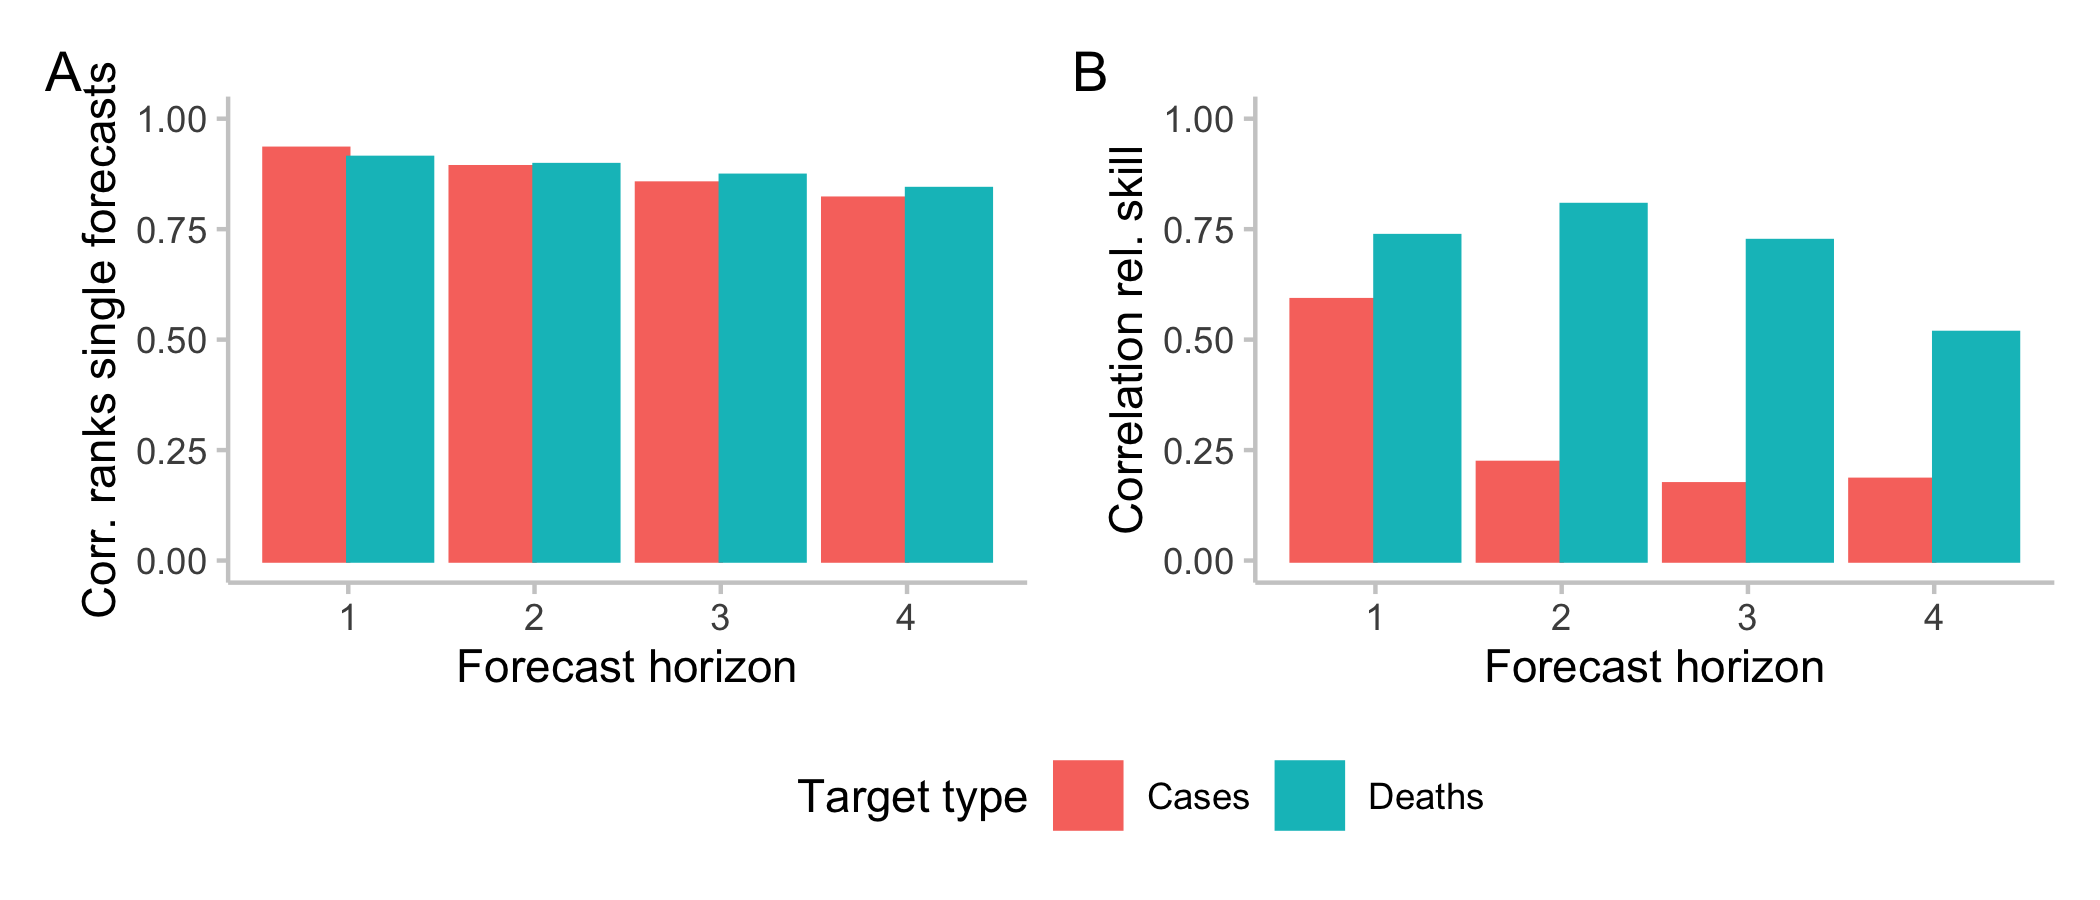
\includegraphics[width=0.9\textwidth]{output/figures/HUB-cors.png}
    \caption{Correlation between scores on the natural and on the log scale. A: Correlation between relative ranks (the rank in terms of WIS divided by the number of models) for individual forecasts, separated by forecast horizon. B: Correlation between relative skill values achieved by models across locations and time points, separated by forecast horizon. SHOULD THIS BE SPEARMAN?}
    \label{fig:HUB-cors}
\end{figure}

When evaluated on the natural scale, there is  strong relationship between the mean of the weighted interval score and the total number of observed cases (correlation: 0.913) or deaths (cor: 0.849) in a location (see Figure \ref{fig:HUB-mean-scores-total-loglog} and Figure \ref{fig:HUB-mean-scores-total} in the SI). The relationship is less pronounced for scores on the log scale (cor: -0.019 for cases, -0.395 for deaths) and negative, meaning that locations with fewer observed cases or deaths tend to receive higher scores. 

\begin{figure}[h!]
    \centering
    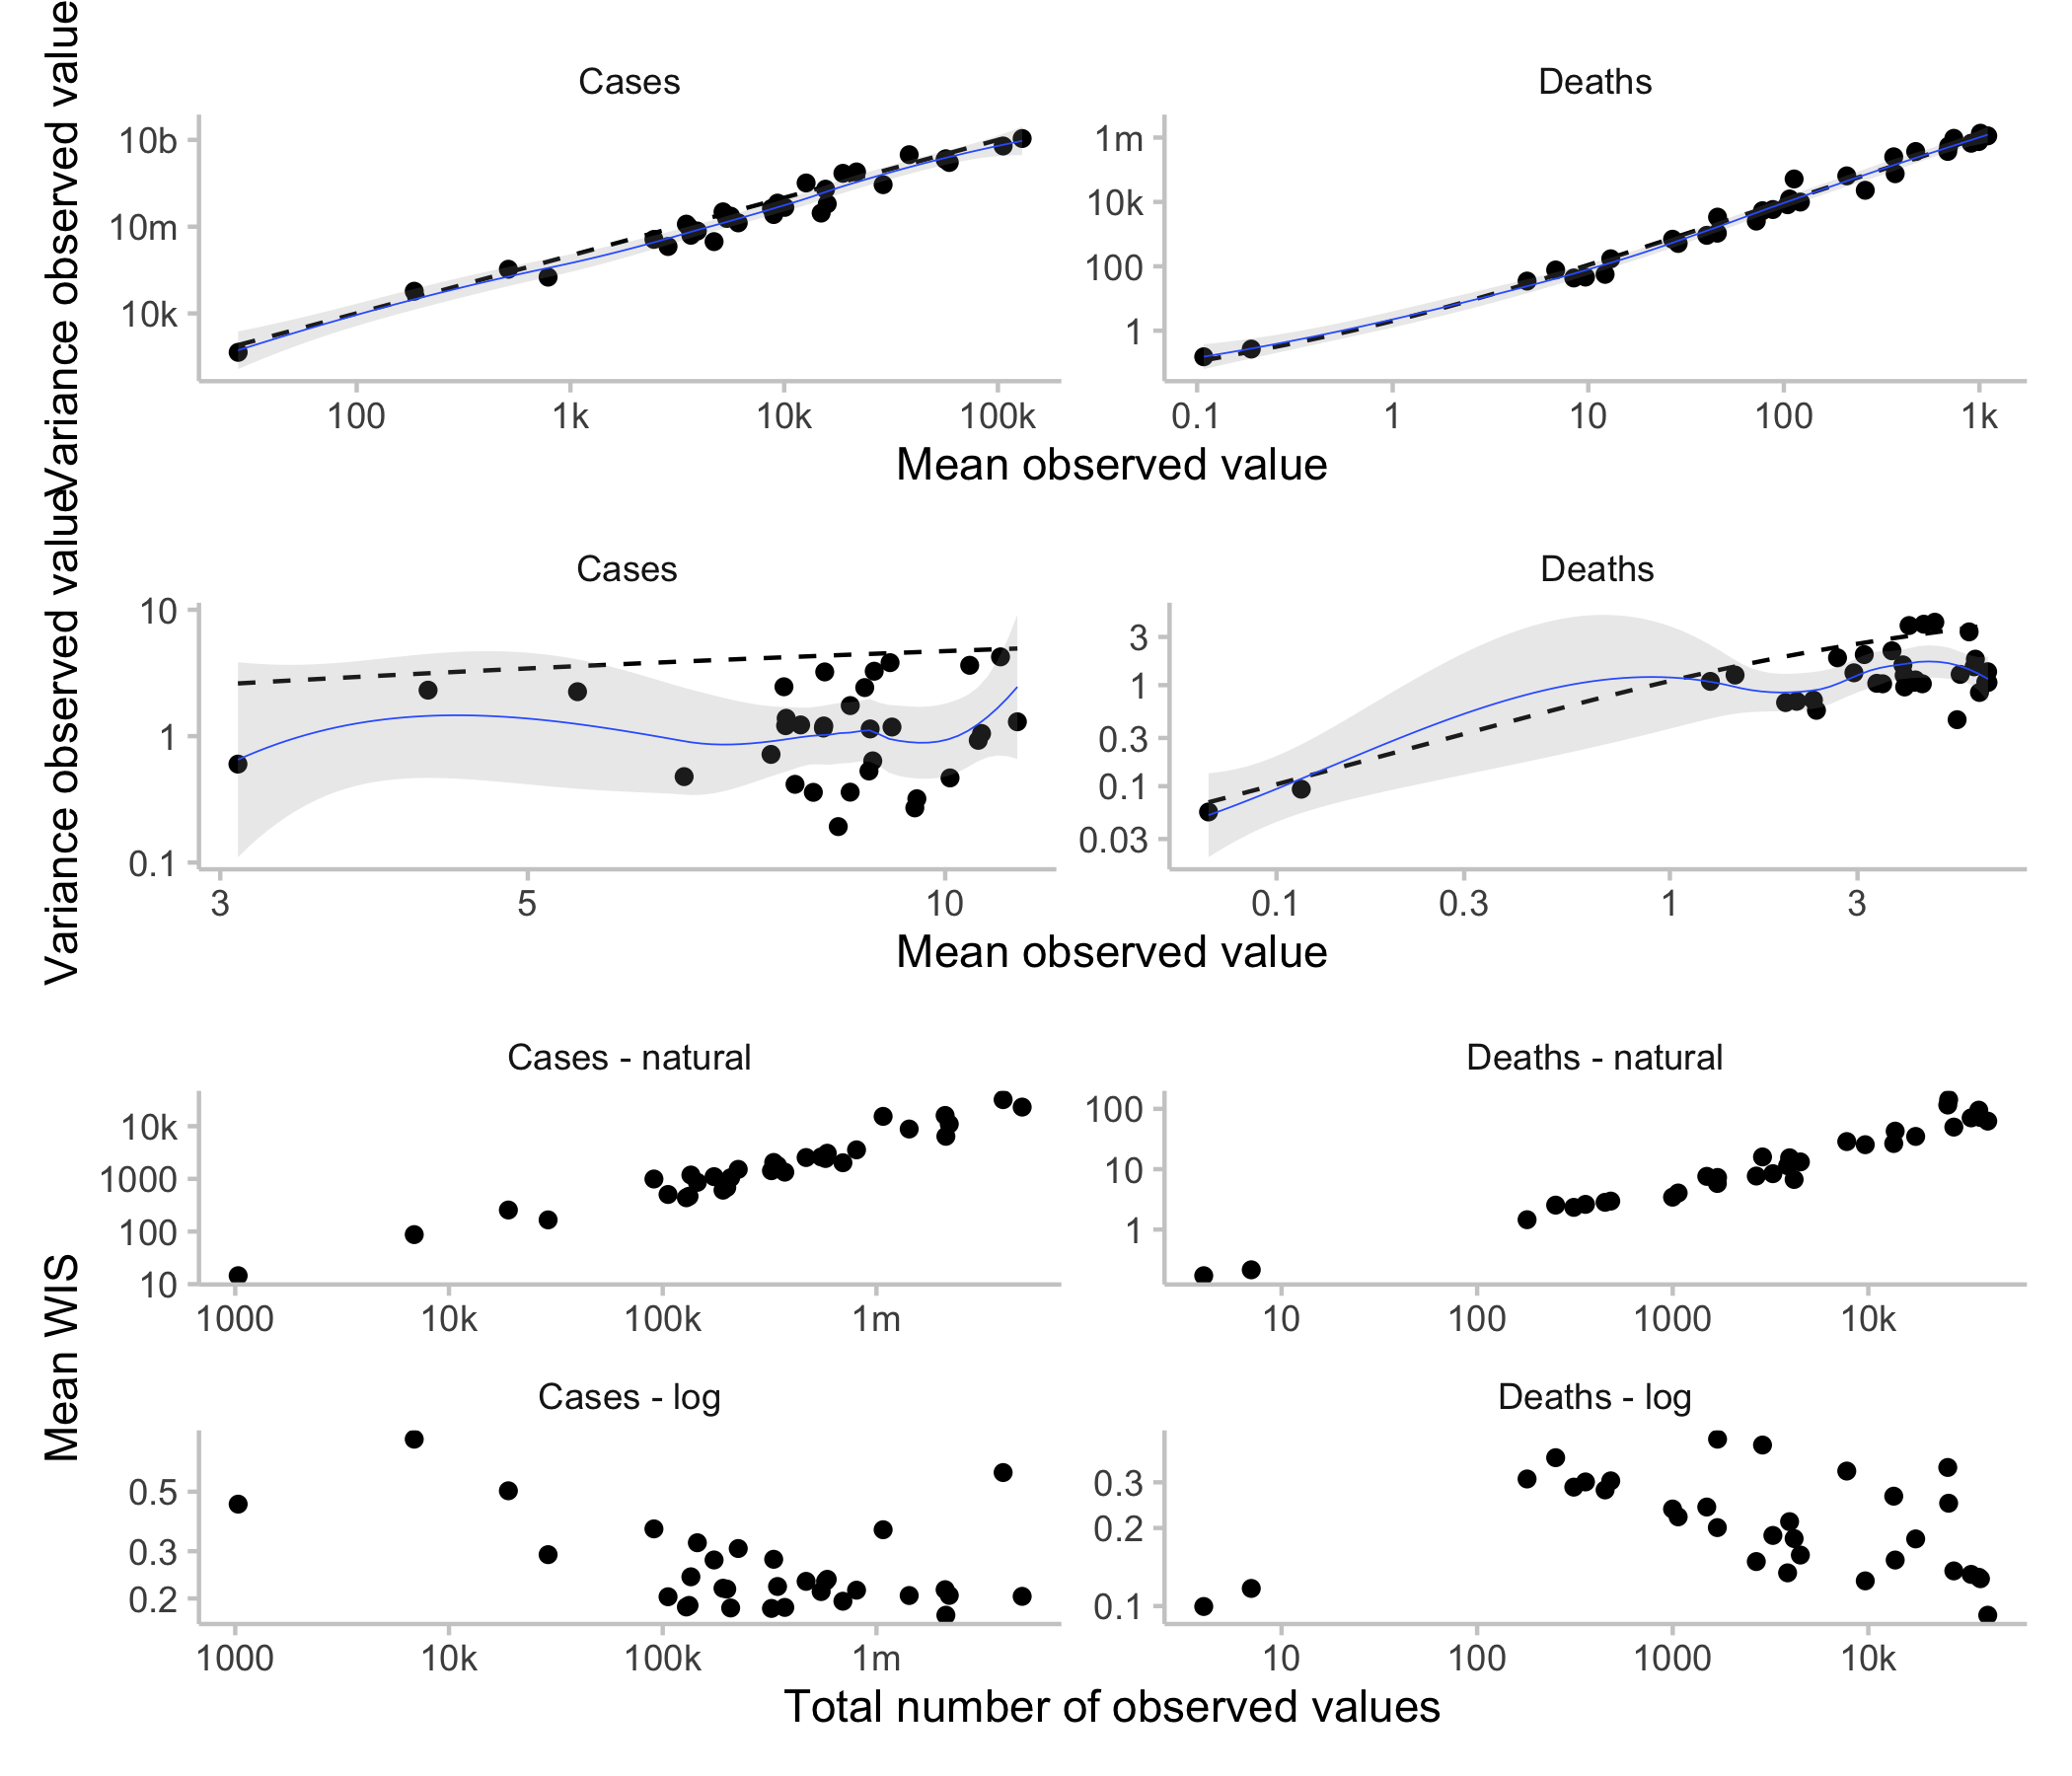
\includegraphics[width=0.9\textwidth]{output/figures/HUB-mean-scores-vs-total-log-log.png}
    \caption{Plot with Weighted interval scores against the mean number of observed cases or deaths.}
    \label{fig:HUB-mean-scores-total-loglog}
\end{figure}

Both on the natural scale as well as on the log scale, scores increase considerably with increasing forecast horizon (see Figure \ref{fig:HUB-scores-horizon}). The increase is more pronounced for cases than for deaths and arguably represents an increase in the relative difficulty to forecast values further into the future. A similar increase both on the natural and the log scale suggests that we are able to observe the increase in difficulty regardless of how we evaluate the scores. 

\begin{figure}[h!]
    \centering
    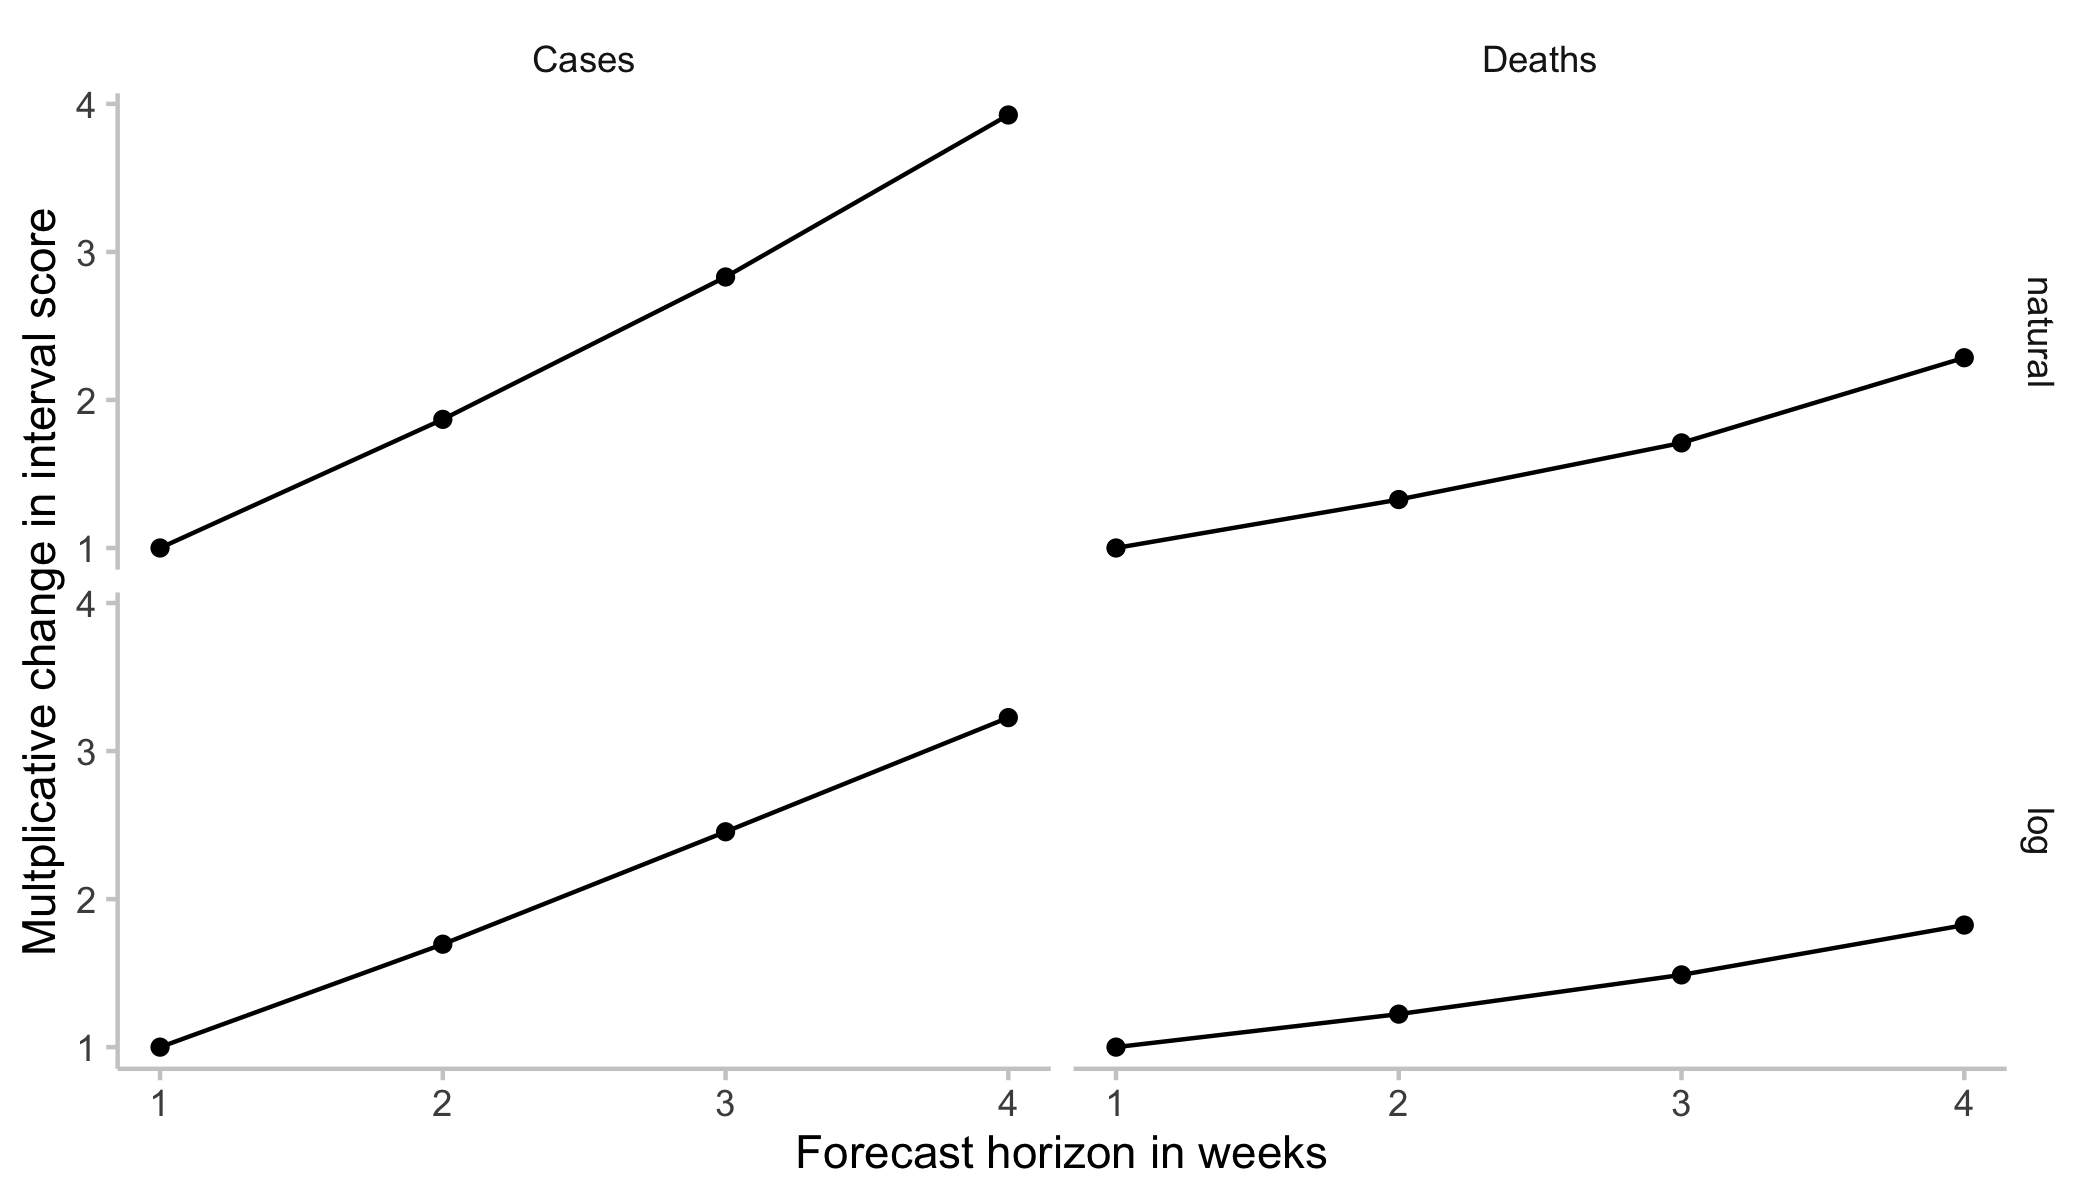
\includegraphics[width=0.9\textwidth]{output/figures/HUB-scores-over-horizon.png}
    \caption{Weighted interval scores across forecast horizons}
    \label{fig:HUB-scores-horizon}
\end{figure}

\paragraph{Rankings}
So one effect is that for a given dispersion on the natural scale, it's better if that interval is skewed, as that implies that at least you only off a lot in one direction in negative terms, and not in the other direction. Maybe looking at over-and underprediction is the key here. 
%ADD SAME PLOT TO SI FOR HORIZON 4. 

\paragraph{pairwise comparisons}
\begin{figure}[h!]
    \centering
    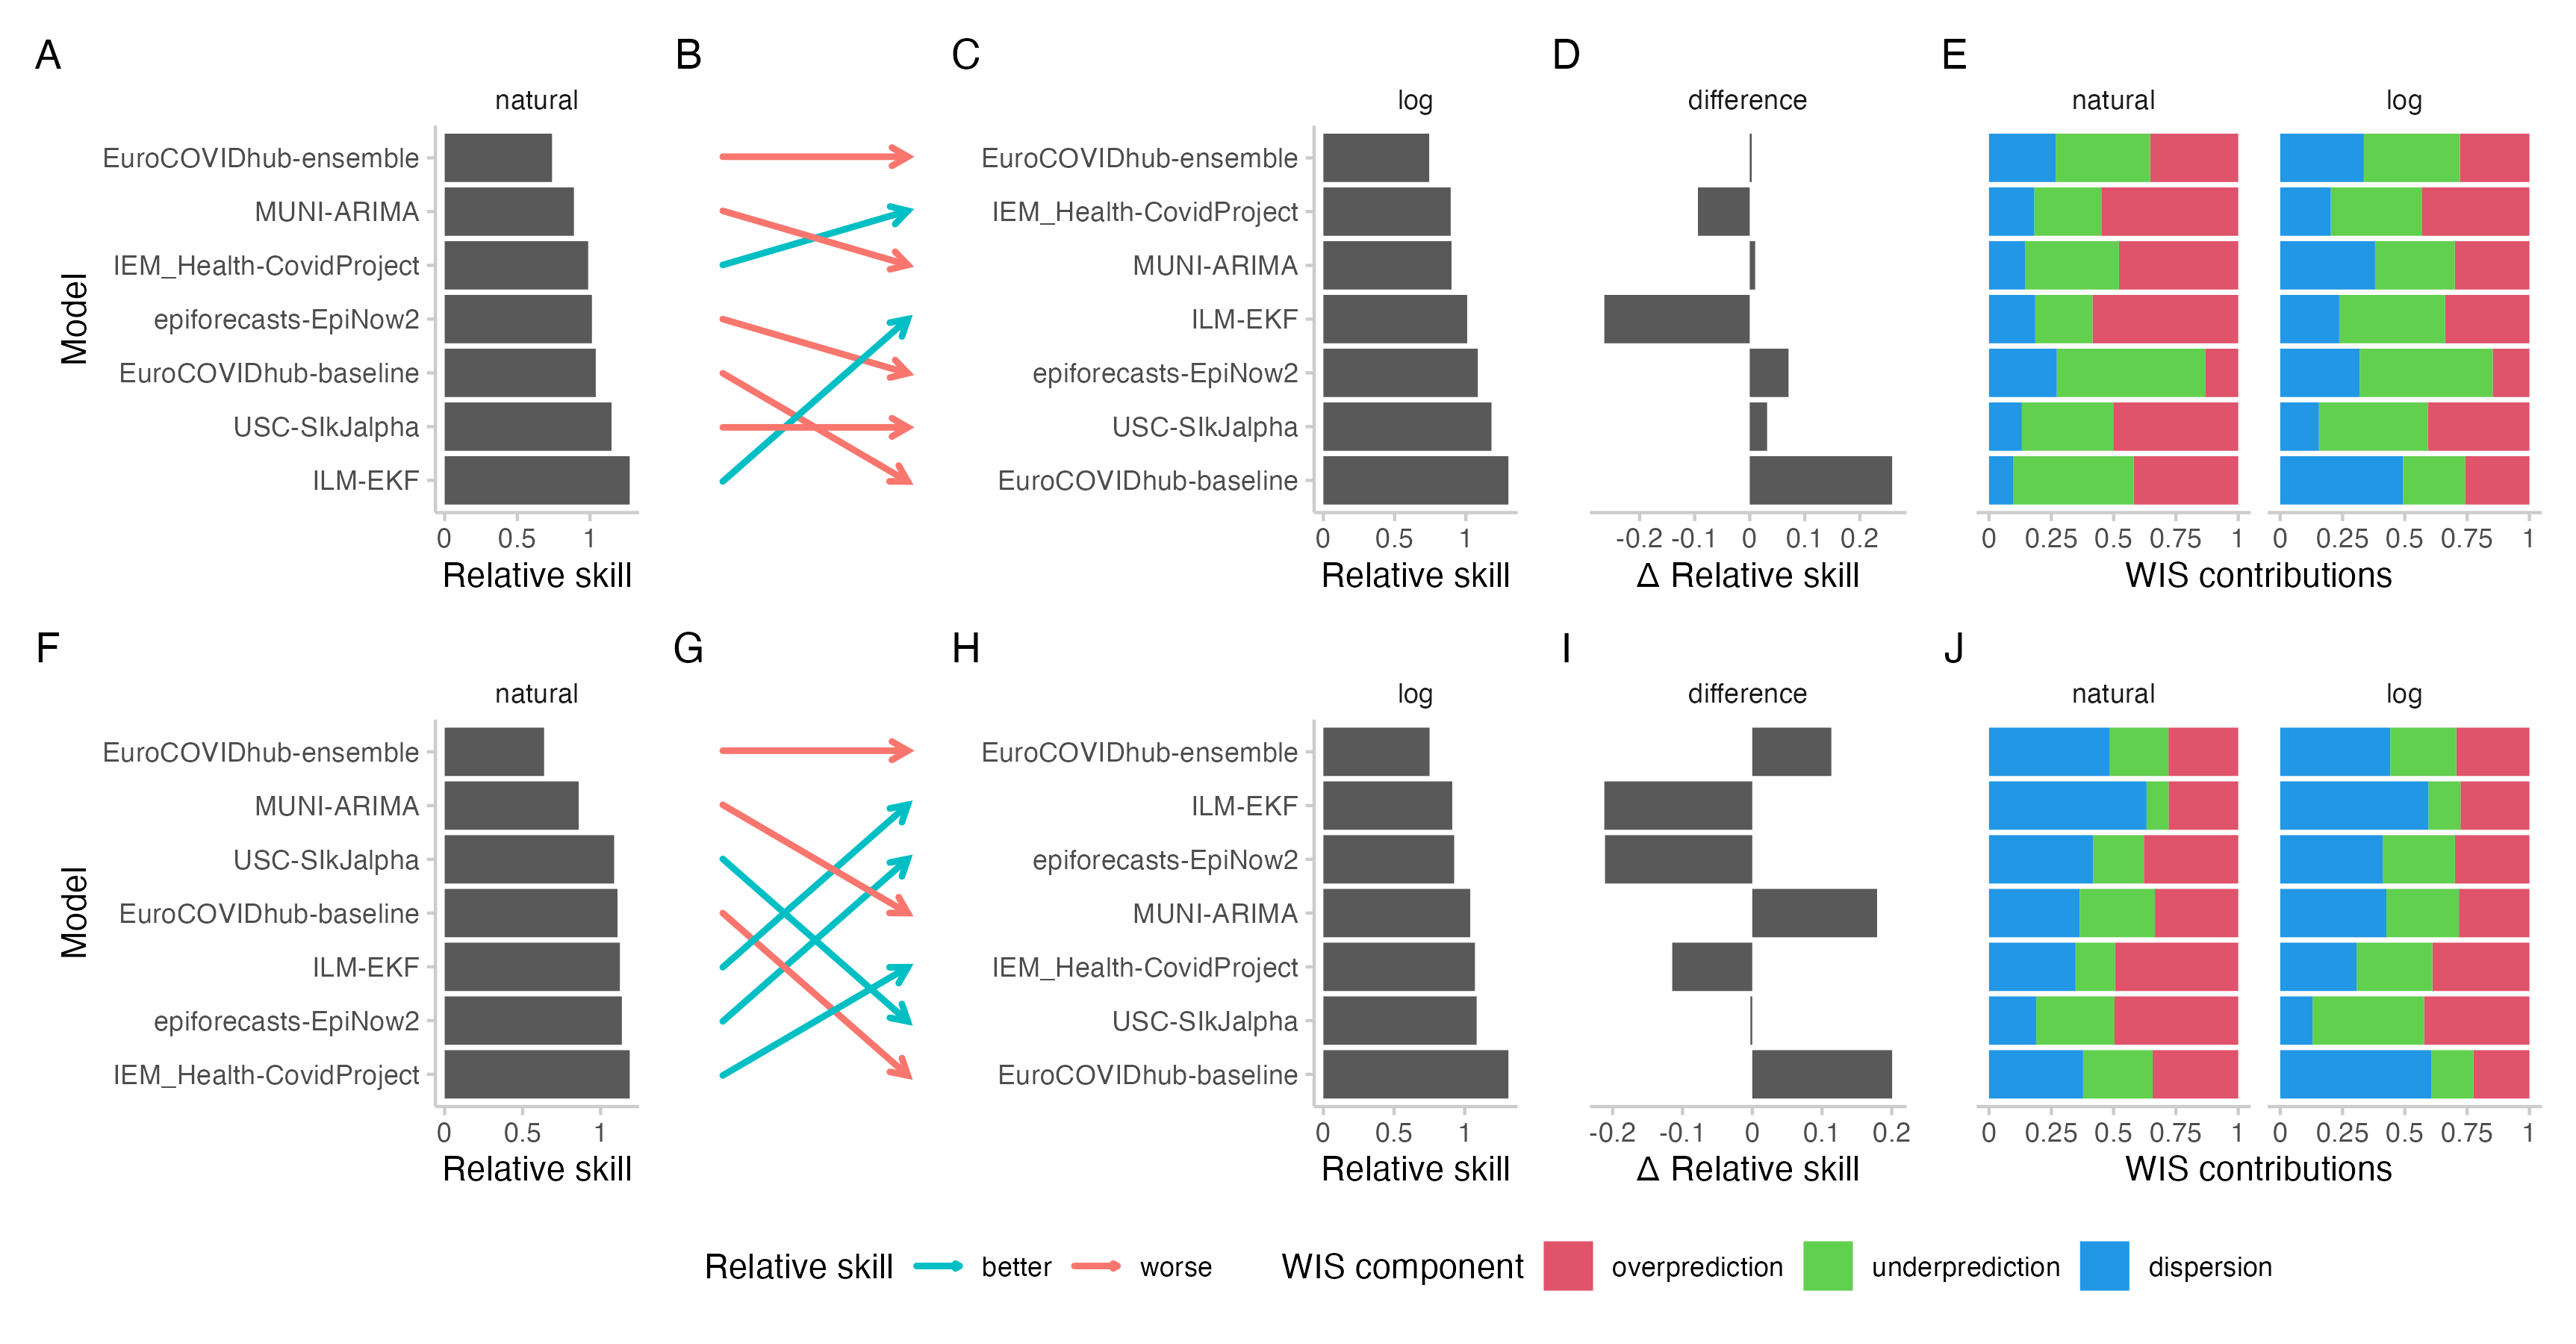
\includegraphics[width=0.9\textwidth]{output/figures/HUB-pairwise-comparisons.png}
    \caption{Changes in relative skill and the distribution of scores}
    \label{fig:HUB-pairwise}
\end{figure}

Correlation between pairwise comparisons is 0.4414717. 



% \section{Other ideas}
% \begin{itemize}
%     \item Compare different predictive distributions and the score as a function of an outcome.
%     \item ...
% \end{itemize}


\begin{figure}[h!]
    \centering
    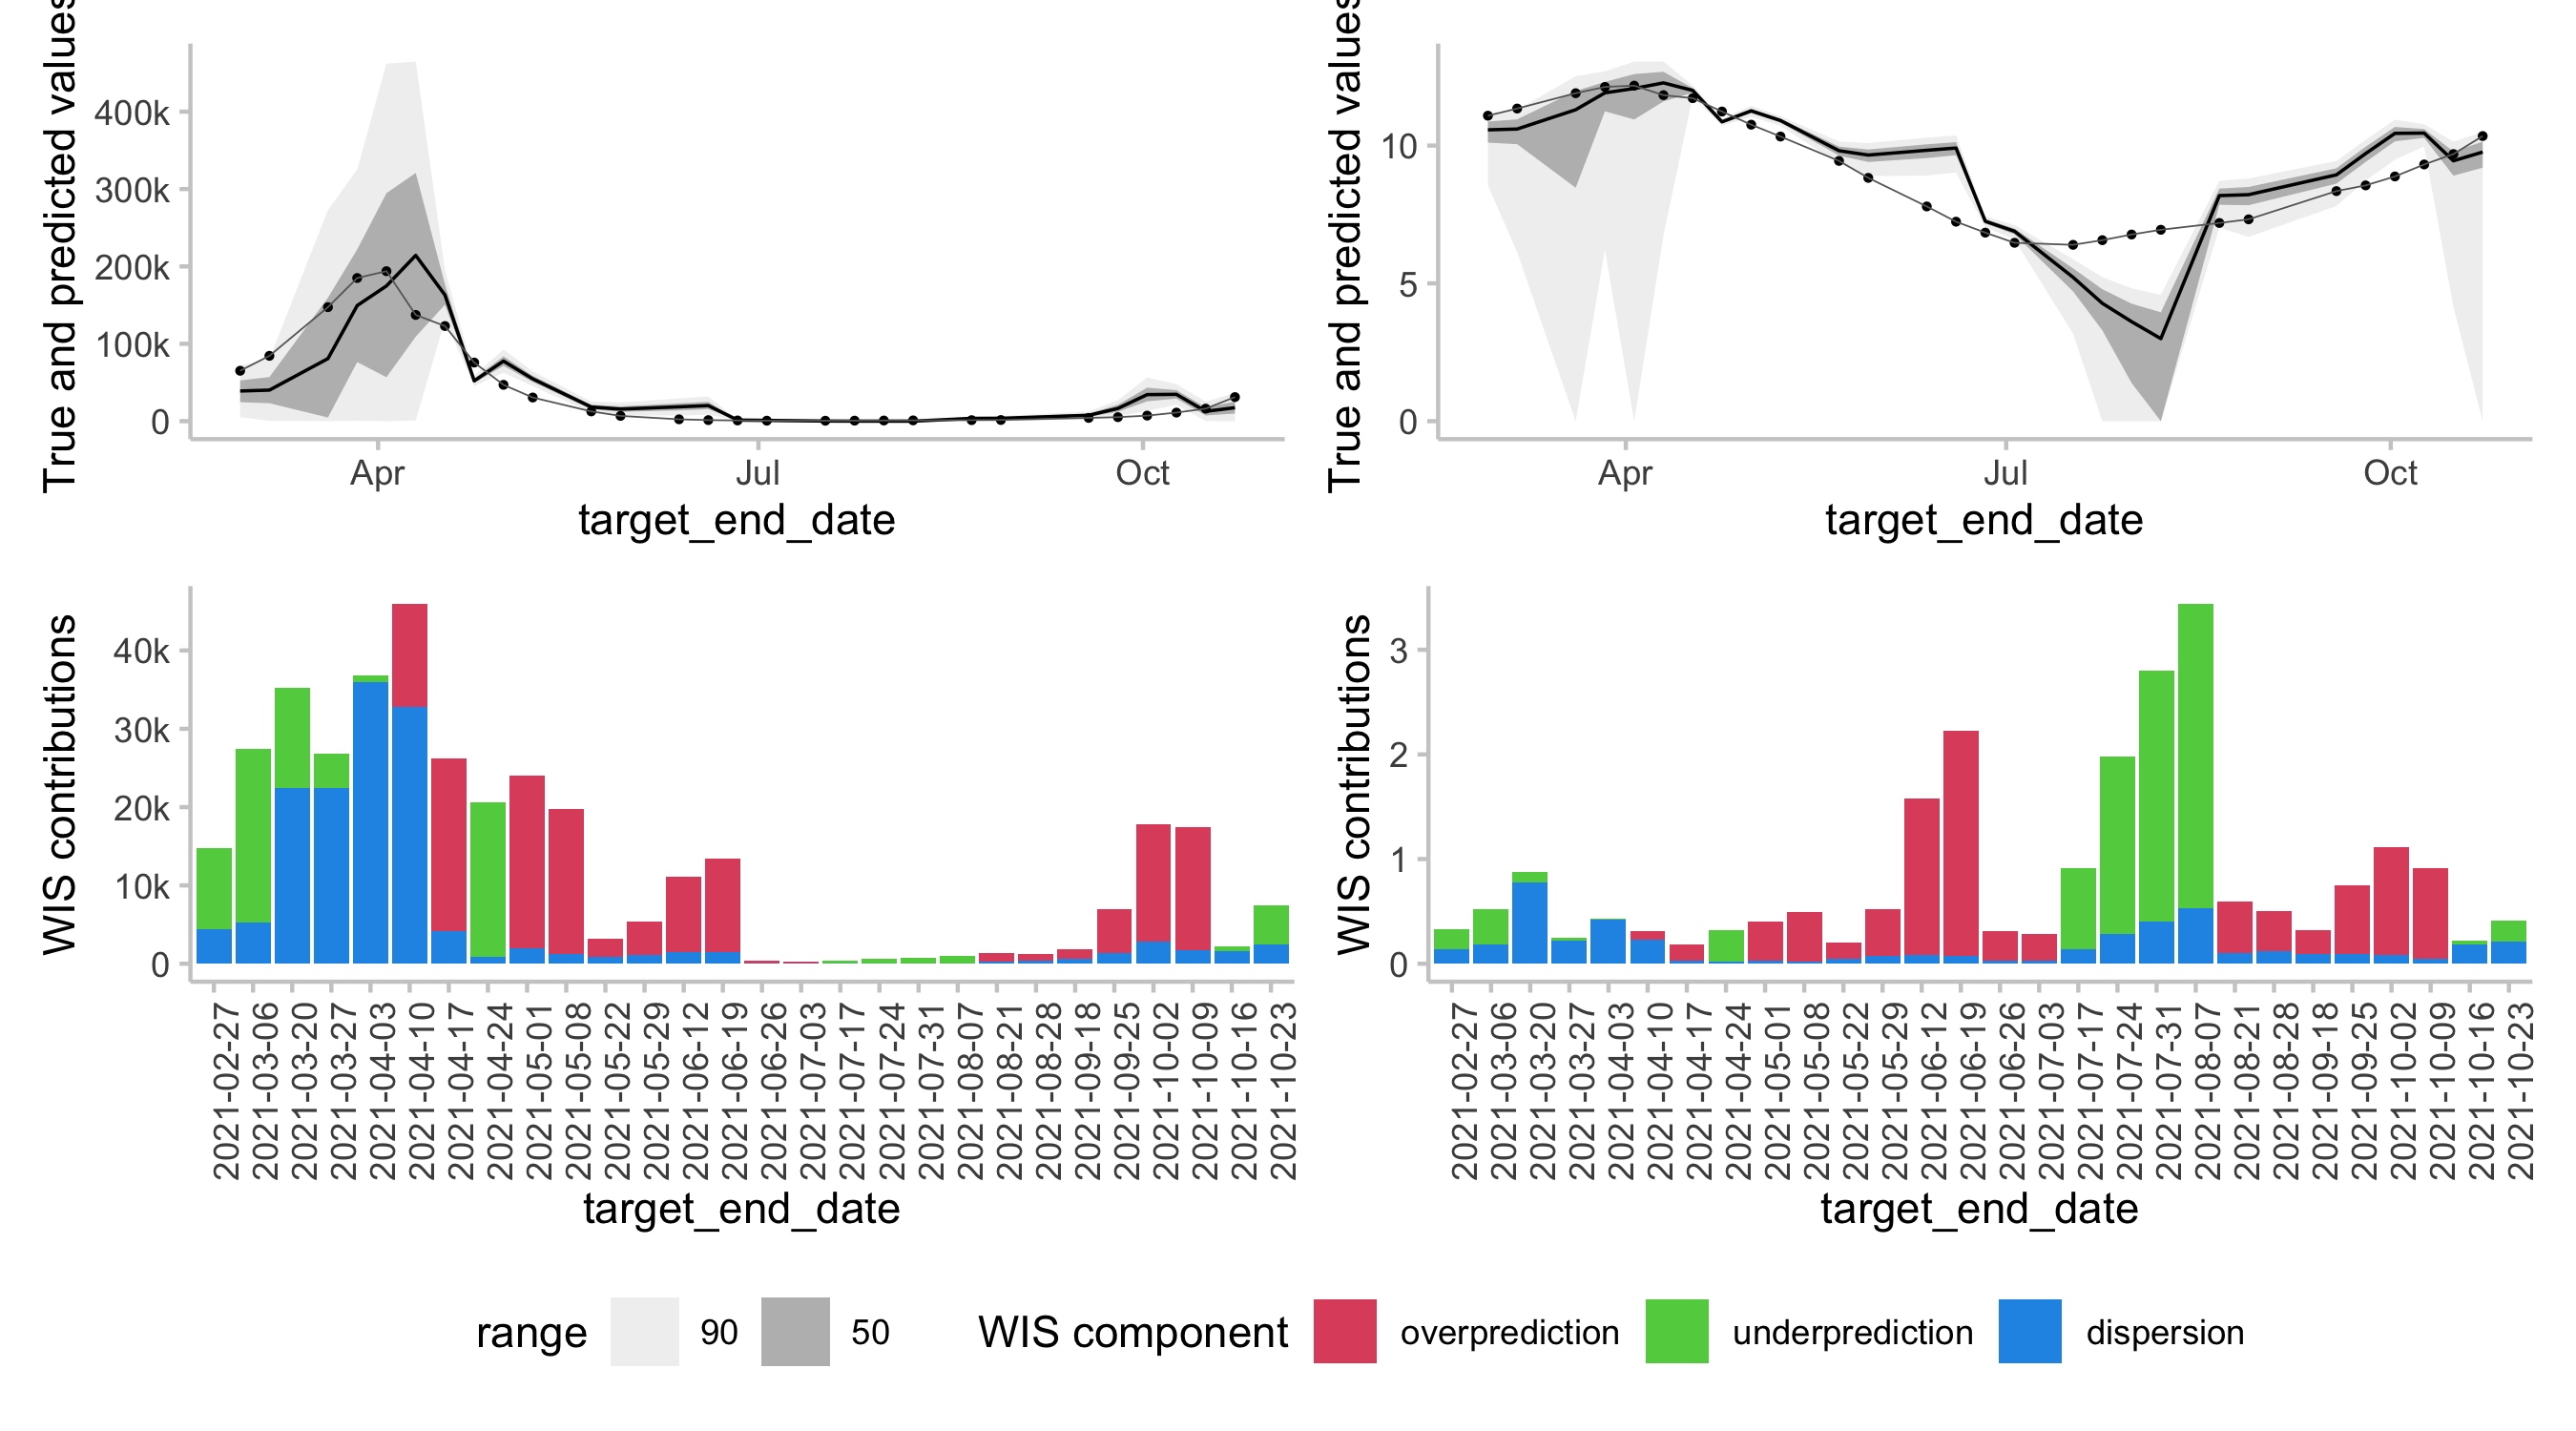
\includegraphics[width=0.9\textwidth]{output/figures/HUB-model-ICM.png}
    \caption{Top: 2-week-ahead predictions. Bottom: scores }
    \label{fig:HUB-model-ICM}
\end{figure}


\begin{figure}[h!]
    \centering
    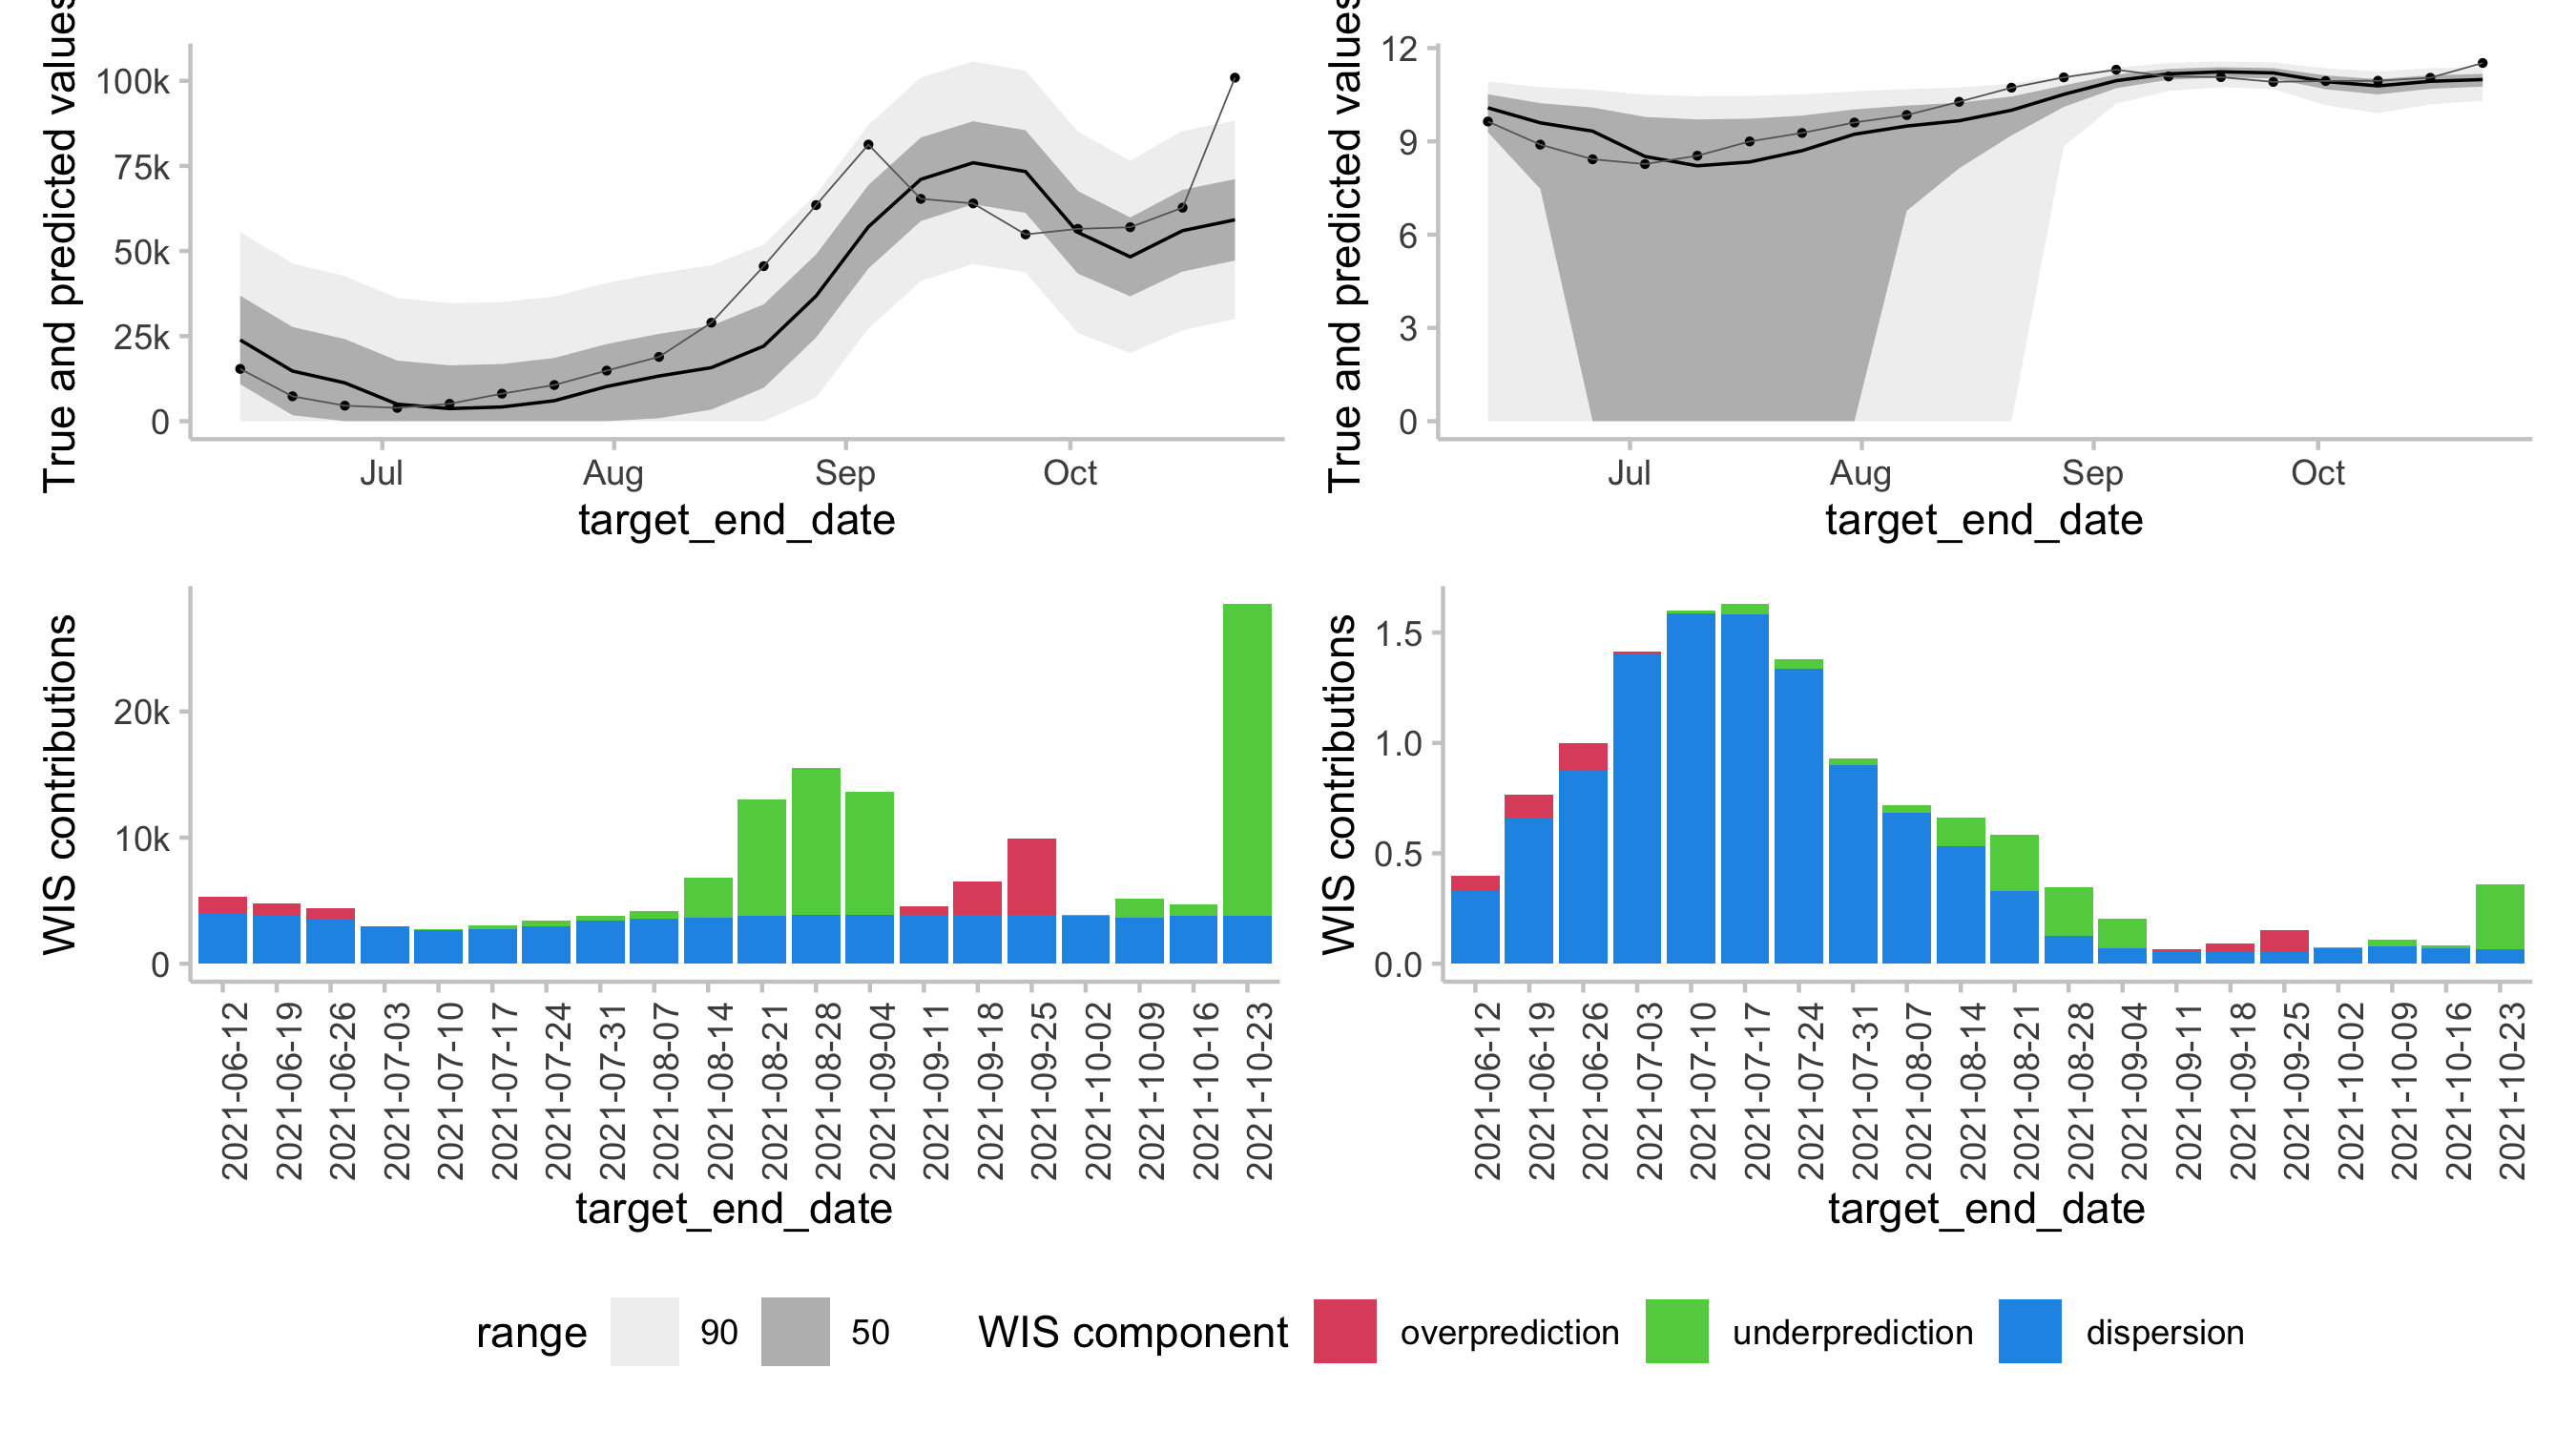
\includegraphics[width=0.9\textwidth]{output/figures/HUB-model-epiBATS.png}
    \caption{Top: 2-week-ahead predictions. Bottom: scores }
    \label{fig:HUB-model-epiBATS}
\end{figure}


\begin{figure}[h!]
    \centering
    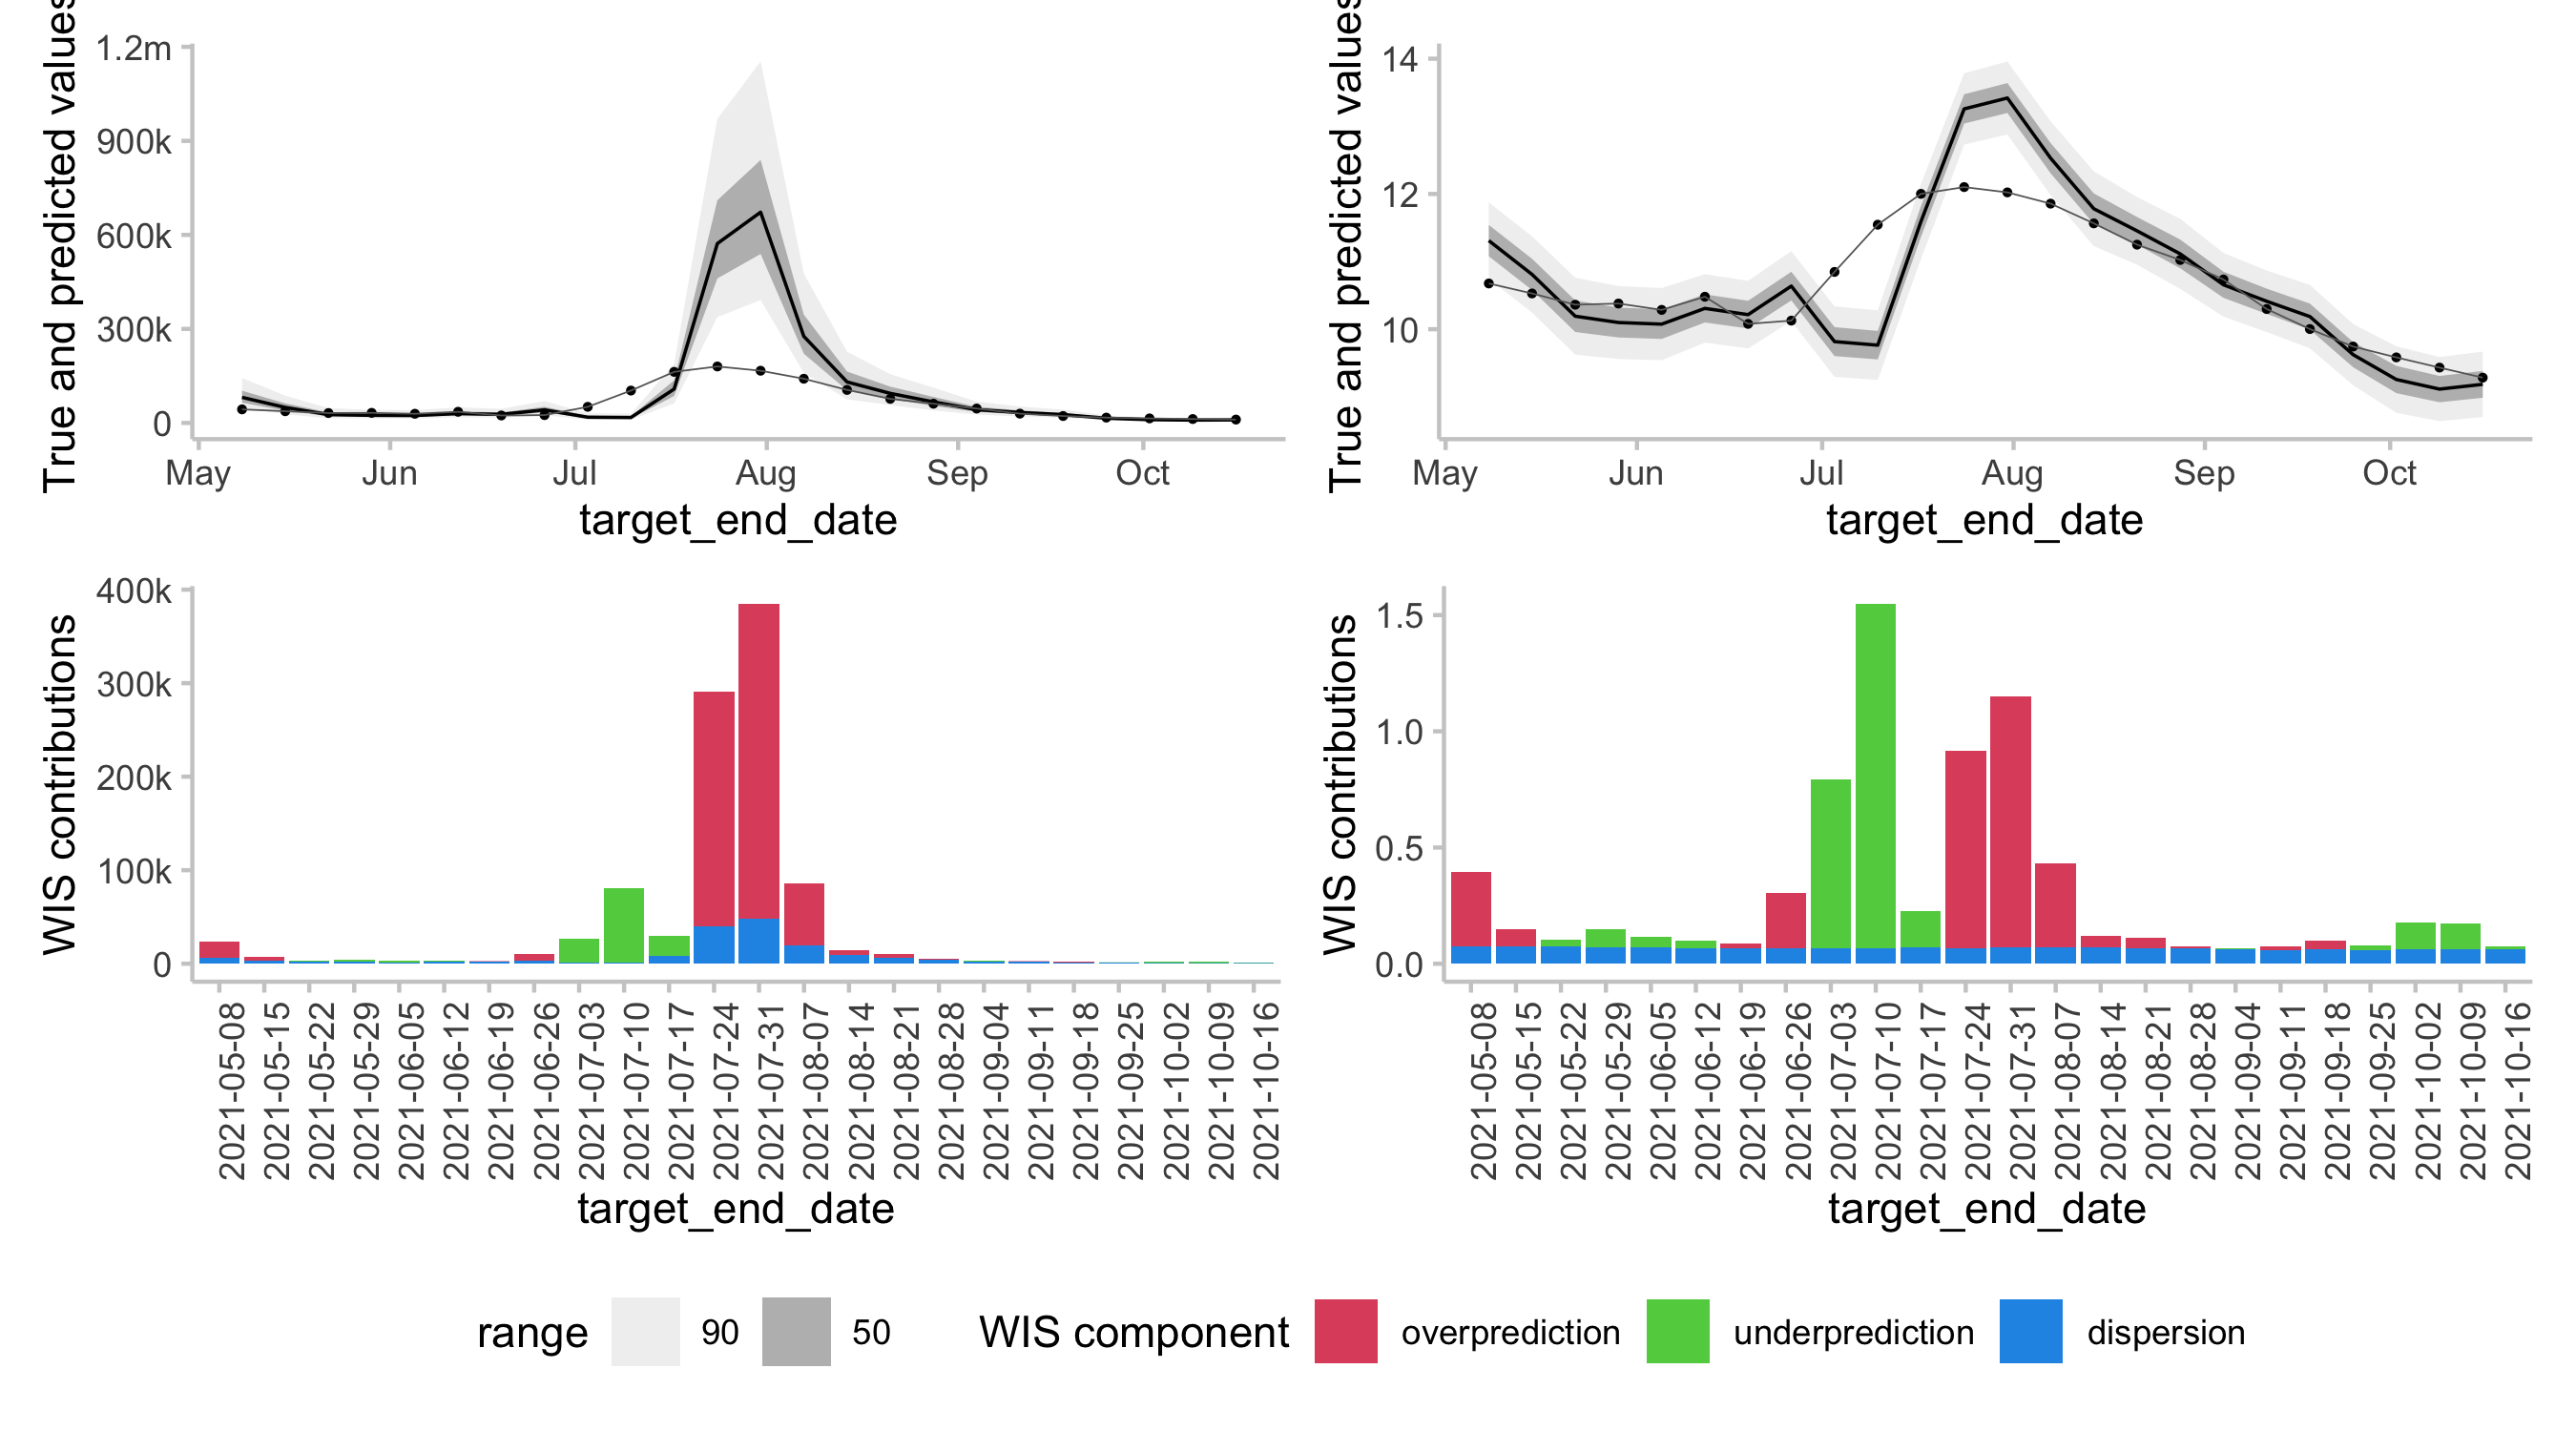
\includegraphics[width=0.9\textwidth]{output/figures/HUB-model-BSLCoV.png}
    \caption{Top: 2-week-ahead predictions. Bottom: scores }
    \label{fig:HUB-model-BSLCoV}
\end{figure}



\section{Discussion}

\paragraph{summary of what we did}
In this paper we suggested that epidemiological forecasts which are today evalaluated using the WIS or CRPS on a natural scale should instead be log transformed first before scoring. This shifts the focus of the evaluation from absolute to relative errors and is a convenient way to score forecasts based on how well they are able to predict the growth rate. This is useful as it makes sure that the evaluation is consistent with the kinds of errors we expect forecasting models to make in an epidemiological context. 

When applied to data from the Europeam Forecasting Hub, we found that 

\paragraph{context, implications, limitations}

SOME DIFFERENCES BETWEEN SCORES ARE MEANINGFUL. E.G. WE WOULDN'T WANT SCORES FOR CASES AND DEATHS TO BE COMPLETELY EQUAL, BECAUSE DEATHS ARE LIKELY EASIER TO FORECAST

\paragraph{outlook, future work}

\paragraph{Other transformations - maybe move to Discussion}
While we focus on the log transformation in this paper, there are other transformations that may be helpful in an epidemiological context. One could for example divide all forecasts by the population in a location, to obtain forecasts standardised incidences per e.g. 100,000 inhabitants. 
Or one could apply a Box-Cox transformation MISSING. 
Or a square-root transformation MISSING. 
Or one could divide each forecast by the forecast of the previous week (and observations by the observation of the previous week), to transform preditions to week-to-week growth rates. This would be akin to evaluating the shape of the predicted trajectory against the shape of the observed trajectory. Note that this is not well defined in the context of forecasts stored as predictive quantiles, as the growth rate of the $\alpha$-quantile may be different from the $\alpha$-quantile of the growth-rate. 



COULD ALSO BE DISCUSSION
Whether or not a log transformation is apprpriate depends on whether one believes that differences in absolute values are meaningful. This may be the case for example when comparing forecasts across locations or time points, rather than different forecasts targets. \cite{bracherEvaluatingEpidemicForecasts2021} for example argue that in epidemiological settings it is a desirable property of the CRPS / WIS that it assigns large scores to forecasts where counts are high, as this naturally reflects the situations we should most care about and helps us identify the models that perform best in similar situations. If, on the other hand, we believe that good models should do consistently well and that situations with high incidences do not provide significantly more information about which models perform well or badly, then scoring on the log scale may be more appropriate. For example, it may be reasonable not to think that predictive performance in a country like Germany would have a hundred times more importance than performance in a country like Luxembourg when determining the best model for future decision making. Similarly, we may not necessarily believe that predictive performance during the January 2022 wave of COVID-19 should carry three times as much weight than predictive performance during the January 2021 wave, just because numbers where three times as high. 


% Divide by the latest known value = score forecast on the growth rate
% - WHAT KINDS OF DATA CAN I CONDITION ON? 
% - WOULD DIVIDING A FORECAST BY ITS RESOLUTION WORK? 
% - CAN I SCORE THE TRAJECTORY / WEEK-TO-WEEK GROWTH RATE BY DIVIDING the 4 week ahead forecast by the three week ahead forecast? 




 %COULD ALSO MAKE A NICE PLOT ABOUT OUTLIERS, where we look at the effect of outliers. but maybe that is already included in the plot in Figure 1. 
% could make an analysis re outliers: how do scores change if we remove the 1 or 2 worst forecasts? The one or two best forecasts?




\newpage

\appendix
\section{Supplementary information}


\subsection{Additional information on the WIS} \label{wis}
\paragraph{WIS}

WIS values are always larger or equal than zero and lower values imply better performance. The WIS can be decomposed into a dispersion component and penalties for over- and under-prediction. For a single prediction interval, the interval score is computed as 
\begin{align}
 IS_\alpha(F,y) &= (u-l) + \frac{2}{\alpha} \cdot (l-y) \cdot 1(y \leq l) + \frac{2}{\alpha} \cdot (y-u) \cdot 1(y \geq u) \\
 &= \text{dispersion} + \text{underprediction} + \text{overprediction},    
\end{align}

where $1()$ is the indicator function, $y$ is the observed value, and $l$ and $u$ are the $\frac{\alpha}{2}$ and $1 - \frac{\alpha}{2}$ quantiles of the predictive distribution $F$, i.e. the lower and upper bound of a single central prediction interval. For a single forecast interval, the interval score is the width of the prediction interval, if it covers the observed value, and the absolute error between the forecast and the lower (or upper, respectively) interval boundary. For a set of $K$ prediction intervals and the median $m$, the WIS is computed as a weighted sum, 
\begin{equation}
\text{WIS} = \frac{1}{K + 0.5} \cdot \left(w_0 \cdot |y - m| + \sum_{k = 1}^{K} w_k \cdot IS_{\alpha}(F, y)\right),    
\end{equation} 
where $w_k$ is a weight for every interval. Usually, $w_k = \frac{\alpha_k}{2}$ and $w_0 = 0.5$. 


The WIS is closely related to the continuous ranked probability score (CRPS) [Cite Gneiting 2007], which itself can be understood as a generalisation of the absolute error to probabilistic forecasts. For an increasing set of equally-spaced prediction intervals the WIS converges to the CRPS and shares many of its properties. More information on the CRPS is provided in section \ref{crps} in the SI. 

\subsection{Additional information on the CRPS} \label{crps}

The CRPS measures the 'distance' of the predictive distribution to the observed data-generating distribution as 

\begin{equation}
    \text{CRPS}(F, y) = \int_{-\infty}^\infty \left( F(x) - 1(x \geq y) \right)^2 dx,
\end{equation}

where y is the true observed value and F the CDF of predictive distribution. Often the following alternative representation is used
\begin{equation}
    \text{CRPS}(F, y) = \frac{1}{2} \mathbb{E}_{F} |X - X'| - \mathbb{E}_P |X - y|,
\end{equation}
  
where $X$ and $X'$ are independent realisations from the predictive distributions $F$ with finite first moment and $y$ is the true value. In this representation we can simply replace $X$ and $X'$ by samples sum over all possible combinations to obtain the CRPS.  





\subsection{Scoring the growth rate directly}
By dividing every observed value and every forecast by the last observed value prior to evaluation, we replace forecasting $y_{t+1}$ with forecasting  $y_{t+1} / y_t = 1 + g_{t, t+1}$. Just as we were previously penalised an additive error with respect the absolute value, we are now penalising an absolute error with respect to the growth rate. 

We can illustrate what's happening by thinking of an analogous point prediction $\hat{g_{t, t+1}}$ for the growth rate. We could then write
\begin{equation}
    1 + g_{t, t+1} = 1 + \hat{g}_{t, t+1} + \varepsilon^*_{t+1}. 
\end{equation}
%
The WIS and CRPS would evaluate the forecast based on the error $\varepsilon^*_{t+1}$. This translates to an absolute error on the actual forecast target that is multiplicatively connected to the last observed value: 
\begin{align}
    y_{t+1} &= (1 + \hat{g}_{t, t+1} + \varepsilon^*_{t+1}) \cdot y_t \\
            &= (1 + \hat{g}_{t, t+1}) \cdot y_t + \varepsilon^*_{t+1} \cdot y_t \\
            &= \hat{y}_{t+1} + \varepsilon^*_{t+1} \cdot y_t.
\end{align}

One disadvantage of this is that we can't really do anything when an observation is zero. 
%is this helpful?%
%Maybe add some math on how we actually transform the distribution. E.g. divide every quantile or sample by the last observed value, divide the distribution?%


\subsection{Changes in the WIS for forecasts on the log scale} \label{wis-log-derivation}

This connection with the underlying epidemic growth rate is an attractive property in and of itself as it is the conceptual target many forecasters and forecast consumers make use of. 

When we score a forecast for $y_{t+1}$ on the log scale, the interval score for a single prediction interval changes as follows
%
\begin{align}
    \text{IS}_\alpha(\log F, \log y) = &(\log u - \log l) \\ 
    &+ \frac{2}{\alpha} \cdot (\log l - \log y) \cdot 1(\log y \leq \log l) \\
    &+ \frac{2}{\alpha} \cdot (\log y - \log u) \cdot 1(\log y \geq \log u).
\end{align}
%
Note that the values of the indicator functions stay the same as the logarithm is a monotonic transformation and the inequality is preserved. 
On the natural scale, $u$, $l$ are the lower and upper bounds of a central prediction interval for a forecast of $y_{t+1} = (1 + g_{t, t+1}) \cdot y_t$. 
We can rewrite these as 
\begin{equation}
   l = l^* \cdot y_t 
   \;\; \text{and} \;\; 
   u = u^* \cdot y_t,  
\end{equation}
where $u^*$ and $l^*$ are the lower and upper bounds of a prediction interval for $(1 + g_{t, t+1})$. Consequently, 
\begin{equation}
  \log l = \log l^* + \log y_t
  \;\; \text{and} \;\;
  \log u = \log u^* + \log y_t. 
\end{equation}
%
We can then rewrite the score for a forecast of $\log y_{t+1} = \log (1 + g_{t,t+1}) + \log y_t$ as
%
\begin{equation}
\begin{aligned}
IS_\alpha&(\log F_{t+1}, \log y_{t+a}) = \\
&((\log u^* + \log y_t) - (\log l^* + \log y_t)) \\
&+ \frac{2}{\alpha} \cdot ((\log l^* + \log y_t) - (\log (1 + g_{t, t+1}) + \log y_t)) 
     \cdot 1((\log (1 + g_{t, t+1}) + \log y_t) \leq (\log l^* + \log y_t) \\
&+ \frac{2}{\alpha} \cdot ((\log (1 + g_{t, t+1}) + \log y_t) - (\log u^* + \log y_t)) 
      \cdot 1((\log (1 + g_{t, t+1}) + \log y_t) \geq (\log u^* + \log y_t),
\end{aligned}
\end{equation}
%
which simplifies to 
%
\begin{equation}
\begin{aligned}
\label{eqn:is-log}
\text{IS}_\alpha(\log F_{t+1}, \log y_{t+a}) = &(\log u^* - \log l^*) \\
&+ \frac{2}{\alpha} \cdot (\log l^* - \log (1 + g_{t, t+1}) 
     \cdot 1(\log (1 + g_{t, t+1}) \leq \log l^*) \\
&+ \frac{2}{\alpha} \cdot (\log (1 + g_{t, t+1}) - \log u^*) 
      \cdot 1(\log (1 + g_{t, t+1}) \geq \log u^*).
\end{aligned}
\end{equation}

The left-hand side of equation \ref{eqn:is-log} was left unchanged. From the right-hand side we can see that for a single prediction interval, scoring the log of a forecast ($\log F_{t+1}$) against the log observed value ($\log y_{t+1}$) is exactly equivalent to evaluating a forecast for $\log (1 + g_{t, t+1})$. With $\log (1 + g_{t, t+1} \approx g_{t, t+1}$, this is approximately a forecast for the growth rate for small values of $g_{t, t+1}$. 


\subsection{Additional figures}




\begin{figure}[h!]
    \centering
    \includegraphics[width=0.9\textwidth]{output/placeholder-image.png}
    \caption{Placeholder}
    \label{fig:placeholder}
\end{figure}


\begin{figure}[h!]
    \centering
    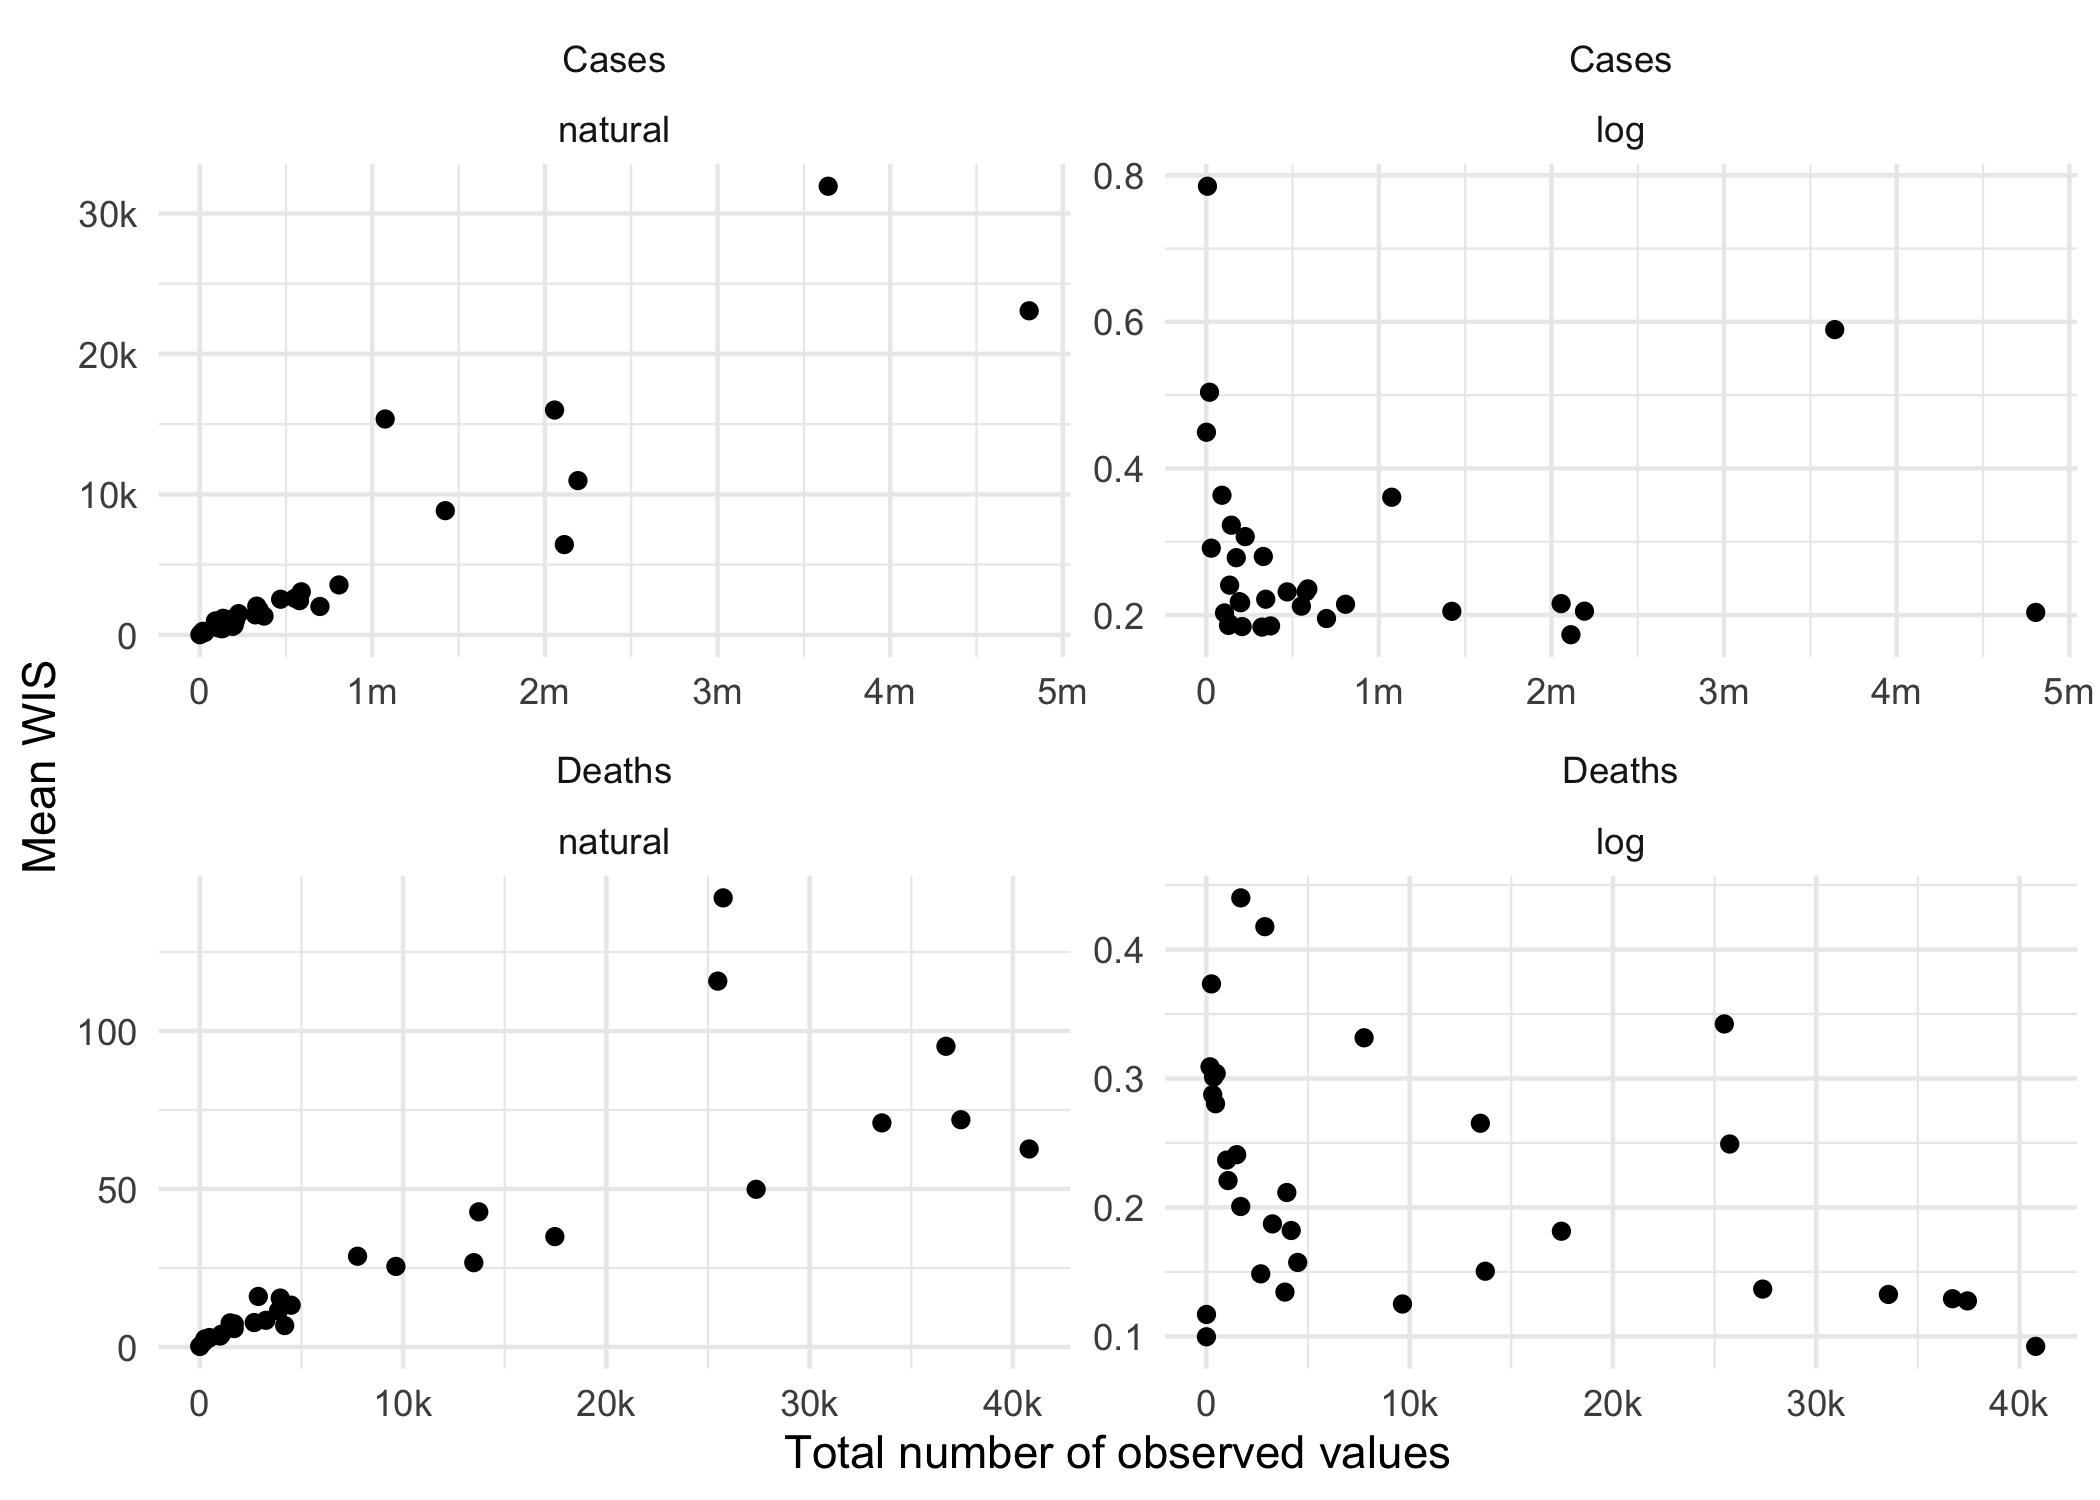
\includegraphics[width=0.9\textwidth]{output/figures/HUB-mean-scores-vs-total.png}
    \caption{Plot with Weighted interval scores against the mean number of observed cases or deaths.}
    \label{fig:HUB-mean-scores-total}
\end{figure}

\begin{figure}[h!]
    \centering
    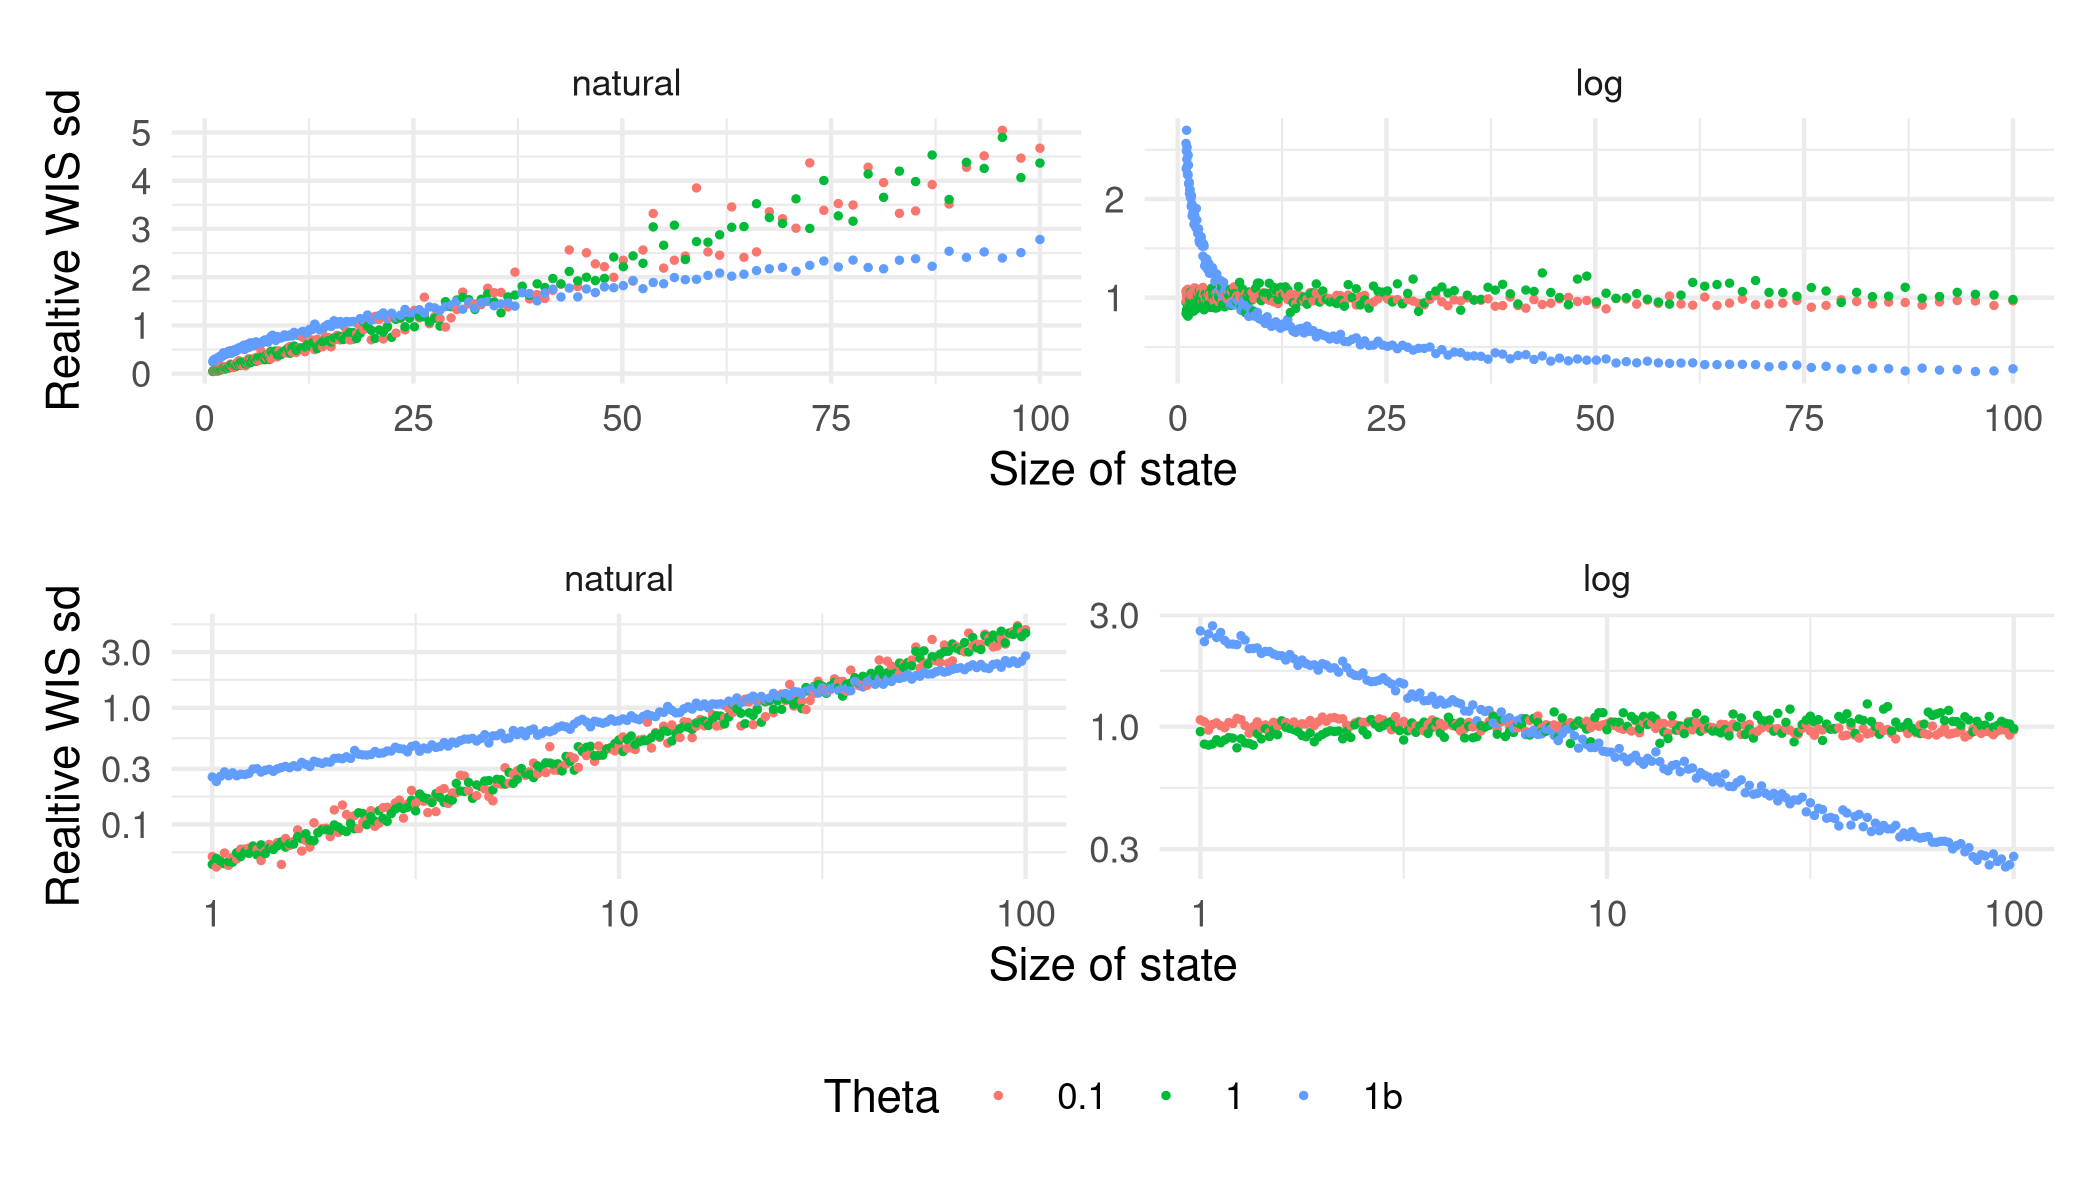
\includegraphics[width=0.9\textwidth]{output/figures/SIM-sd-state-size.png}
    \caption{Simulation of the effect of population size with ideal forecasts of a negative-binomially-distributed variable. For each simulated state, we drew 1,000 observations from a negative binomial distribution with $\mu = 100 \cdot \text{state size}$ and with values of $\theta$ equal to 0.1, 1, and 1 billion. The variance of the negative binomial is given as $\sigma^2 = \mu + \mu^2 / \theta$, meaning that for large theta the negative binomial distribution is equal to the poisson distribution. For these simulated values we computed the WIS for an ideal forecast (i.e. the predictive distribution was negative binomial with $\mu$ and $\theta$ equal to the true $\mu$ and $\theta$ for every state). Left: Mean WIS depending on state size, right: Mean WIS depending on state sizes when scored on a log scale. Plots for the standard deviation, rather than the mean of WIS values look are given in Figure \ref{fig:SIM-wis-state-size-sd} in the SI.}. 
    \label{fig:SIM-wis-state-size-mean}
\end{figure}


\bibliography{log-or-not.bib}


\end{document}


%%%%%%%%%%%%%%%%%%%%%%%%%%%%%%%%%%%%%%%%%%%%%%%%%%%%%%%%%%%%%%%%%%%%%%%%%%%%
% Idea parking lot 
%%%%%%%%%%%%%%%%%%%%%%%%%%%%%%%%%%%%%%%%%%%%%%%%%%%%%%%%%%%%%%%%%%%%%%%%%%%%

% NOT SO CONVINCED ANYMORE THAT THIS WORKS. MY INTUITION IS IF YOU WANT THE GROWTH RATE YOU SHOULD ACTUALLY SCORE THE GROWTH RATE AND DIVIDE BY THE LAST OBSERVED VALUE. 
% 
% WELL MAYBE IT WORKS AFTER ALL AND IT WOULD BE THE EQUIVALENT OF LOGGING FIRST AND THEN SUBTRACTING THE LAST OBSERVED VALUE WAIT A MINUTE THAT'S A DIFFERENT TRANSFORMATION AND ALSO THAT's SCORING THE LOG GROWTH RATE. 
% 
% BUT THEN AGAIN I'M STILL CONFUSED, BECAUSE ANY RELATIVE ERROR ON A QUANTITY Y\_t+1 IS AUTOMATICALLY AN ABSOLUTE ERROR ON THE GROWTH RATE IF WE KNOW Y\_t. AH BUT YOU DON'T KNOW WHAT THE ABSOLUTE ERROR ON THE GROWTH RATE IS (E.G. FOR Y\_t+1 of 10 IF YOU DON'T SPECIFICALLY LOOK AT THE LAST VALUE. BUT WE ARE ASSUMING THAT THIS IS WHAT THE MODEL DOES WHEN IT MAKES A FORECAST INTERNALLY




% The WIS can be thought of as an approximation of the CRPS for forecasts where the predictive distribution is represented through a set of quantiles. The CRPS, and by extension the WIS, represents a generalisation of the absolute error to continuous distributions, meaning that forecasters are evaluated on the absolute distance of their predictive distribution to the observed value (i.e. some form of absolute error). For simplicity, we will use absolute error and absolute distance between forecast and observation interchangeably, even though the former applies to point predictions and the latter is used for probabilistic forecasts. 


% 
% 
% 
% We argue that when dealing with epidemiological processes it makes sense to shift the evaluation towards multiplicative errors by either taking the logarithm of both the forecast and the observations or by dividing them by the last known observation before scoring. 

% What kinds of transformations can be considered meaningful depends on the context. We will illustrate the idea of transforming forecasts by focussing on the WIS as it is currently used in epidemiological settings such as the COVID-19 Forecast hubs. 
% In this paper we focus on the WIS due to its simplicity and widespread use by the COVID-19 Forecast Hubs, but arguments apply analogously to the CRPS. Another proper scoring rule commonly used is the log score [CITATION], which we will not discuss further in this paper. 


% \paragraph{Problems with the WIS and CRPS in an epidemiological setting}
% Their relation to the absolute error means that both the WIS and the CRPS usually scale with the prediction target. Forecasts of COVID-19 cases, for example typically have higher scores than forecasts of hospitalisations of death. Similarly, when looking at performance across different locations or over time, average scores will be dominated by locations and times with high incidences. Outliers also can have a disproportionate effect on aggregate scores. One can argue that this is meaningful and that we should care most about places and periods when incidence is high (maybe cite Bracher et al.). However, this may not always be true and is clearly not desirable when comparing performance of a model on different prediction targets: case numbers are not necessarily more important than hospitalisations, just because observed values tend be an order of magnitude higher. This makes forecasts often hard or impossible to compare. 


% not sure this plot is really meaningful
%\begin{figure}[h!]
%    \centering
%    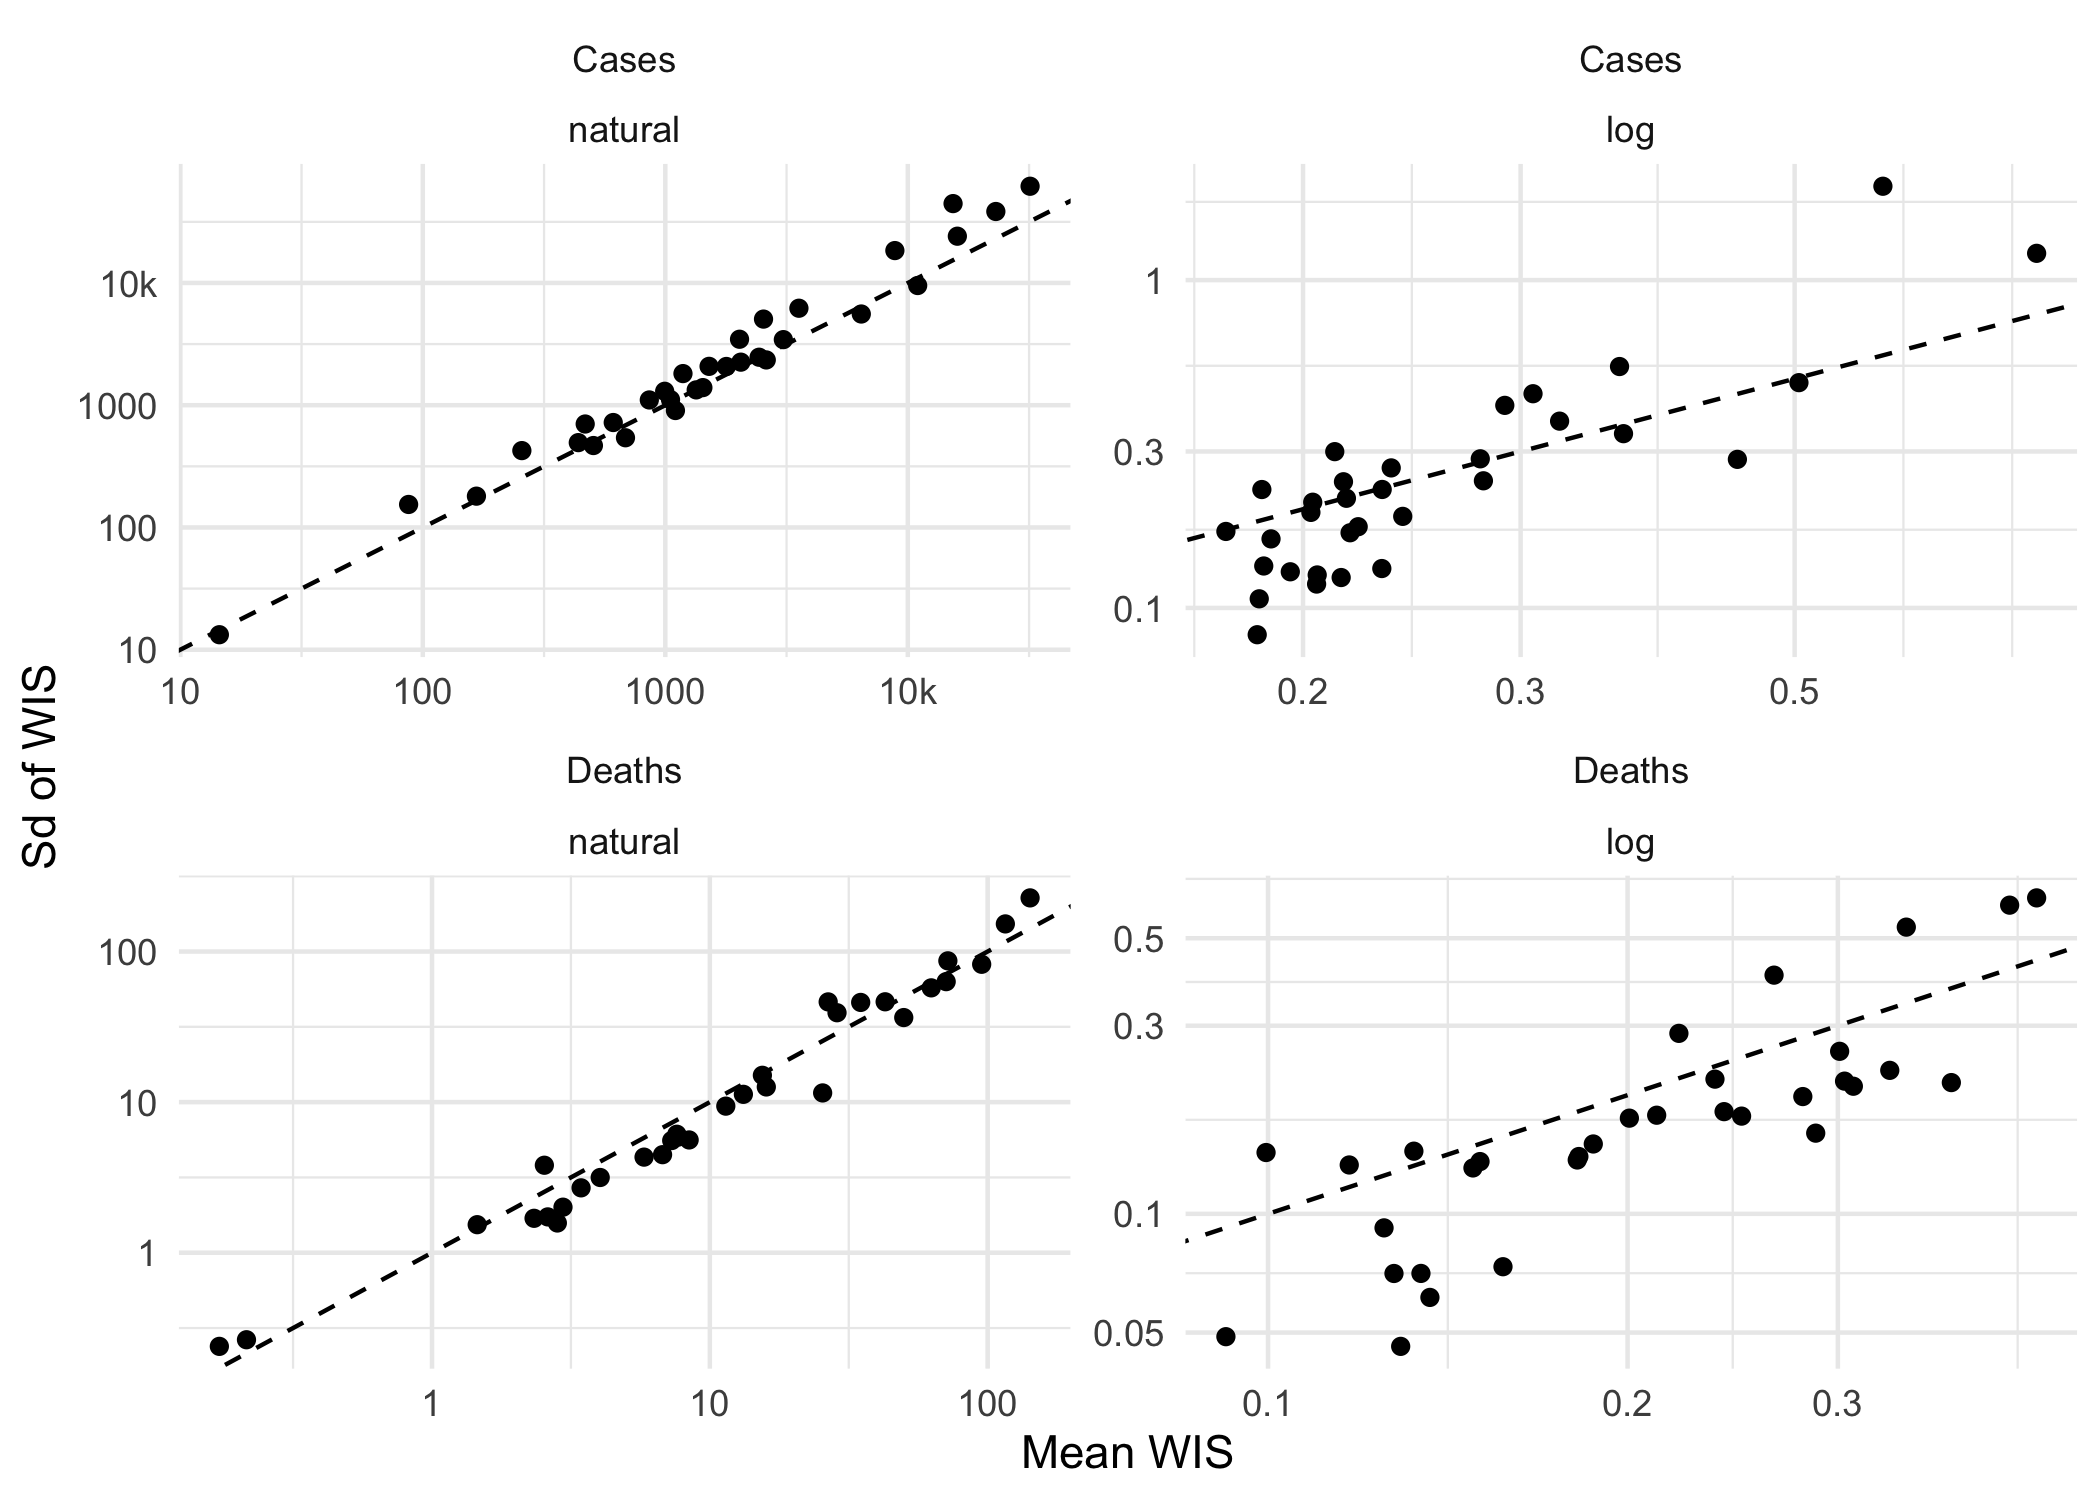
\includegraphics[width=0.9\textwidth]{output/figures/HUB-sd-vs-mean-scores.png}
%    \caption{CAPTION}
%    \label{fig:HUB-mean-sd-scores}
%\end{figure}

%\begin{itemize}
%    \item idea of scores on logged data: interpretation as a measure of relative improvement, just as when you log the absolute error
%\end{itemize}

%\paragraph{What's there in the literature}

%\paragraph{Current problems / questions about scoring an epidemiological setting}
%probably narrow down to the ones we really want to discuss%
%There are limitations with what we can do with scores on a natural scale and open questions whether we can do these things on a log-scale and also whether a log-scale might be inherently more appropriate
%\begin{itemize}
    %\item Can't really model score on a natural scale as errors are heavily skewed. Is there a way to model scores to get insight about different factors that systematically influence scores
 %   \item make a plot somewhere that shows the distribution of scores
  %  \item Maybe epidemiological forecasts are inherently better suited to be scored on an absolute scale due to the multiplicative nature of processes (related to over-prediction > under-prediction)? Does the log-scale imply we are scoring the growth rate? 
   % \item unclear what trade-offs of logging / not logging are
    %\item what score (log, not log) matches closest what our intuition (or policymakers) think is good? 
    %\item are we better at forecasting deaths than cases? --> relative measure would help
    %\item There exists confusion about what can be done to a score in general (e.g. people want to take the median, which they shouldn't) %maybe don't add as an extra point
%\end{itemize}


%\paragraph{Over- and under-prediction}
%If we want to keep this in, we could: 
%\begin{itemize}
%    \item Check whether there is actually a problem with over-prediction and under-prediction in the Hub. This could be the case because we are most interested in certain scenarios in which this might arise. 
%    \item Discuss this in light of Johannes' analysis of how the decomposition of WIS values differs if the data are skewed
%    \item compare this to the PIT-value-like relative bias scores we used for the German / Polish paper, which capture a relative tendency to over- or under-predict, rather than absolute penalties. 
%\end{itemize}


%\section{Modelling scores}
%\paragraph{Motivation} Alternative is to use summary measures or pairwise comparison, which becomes cumbersome for many dimensions. 

%\paragraph{caveats, practical limitations}
%\begin{itemize}
%    \item What kind of transformations can we do? Propose random effect models
%    \item is there anything we can't do? 
%    \item How does logging change the error distribution? On the natural scale, you have huge outliers. What's the appropriate error distribution to use? confidence intervals. Maybe we can only say something about the effects
%\end{itemize}


%\paragraph{Optional: Application to data from the Euro-Hub}
%Also: what, empirically is the distribution of errors? 